%% Käytä toinen näistä:
%% ensimmäinen, jos käytät pdflatexia, joka kääntää tekstin suoraan 
%% pdf-tiedostoksi (kuvat on oltava jpg- tai pdf-tiedostoina)
%% toinen, jos haluat tuottaa ps-tiedostoa (käytä eps-formaattia kuville,
%% alä käytä ps-muotoisia kuvia!)


%% Käytä näitä, jos kirjoitat englanniksi. Katso englanninokset tiedostosta
%% thesistemplate.tex.
\documentclass[english,12pt,a4paper,pdftex,elec,utf8]{aaltothesis}
%\documentclass[english,12pt,a4paper,dvips]{aaltothesis}

\usepackage{graphicx}
\usepackage[binary-units=true]{siunitx}
%\sisetup{detect-family}
%\AtBeginDocument{\sisetup{math-rm=\mathrm, text-rm=\rmfamily}}

%% Matematiikan fontteja, symboleja ja muotoiluja lisää, näitä tarvitaan usein 
\usepackage{amsfonts,amssymb,amsbsy}

\usepackage{listings}
\usepackage[super]{nth}
\usepackage{csquotes}
\usepackage{tikz}
\usetikzlibrary{shapes,arrows}
\usetikzlibrary{dsp, chains}
\usetikzlibrary{arrows, decorations.markings}
\DeclareMathAlphabet{\mathpzc}{OT1}{pzc}{m}{it}
\newcommand{\z}{\mathpzc{z}}
\usepackage{pgfplots}
\usepackage{amsmath,bm,times}
\newcommand{\mx}[1]{\mathbf{\bm{#1}}} % Matrix command
\newcommand{\vc}[1]{\mathbf{\bm{#1}}} % Vector command

\renewcommand{\labelenumii}{\theenumii}
\renewcommand{\theenumii}{\theenumi.\arabic{enumii}.}

\newcommand{\Clanguage}{\lstset{
  language=C++,                % choose the language of the code
  basicstyle=\ttfamily,
  %numbers=left,                   % where to put the line-numbers
  %stepnumber=1,                   % the step between two line-numbers.        
  %numbersep=5pt,                  % how far the line-numbers are from the code
  %backgroundcolor=\color{white},  % choose the background color. You must add \usepackage{color}
  %showspaces=false,               % show spaces adding particular underscores
  %showstringspaces=false,         % underline spaces within strings
  %showtabs=false,                 % show tabs within strings adding particular underscores
 % tabsize=2,                      % sets default tabsize to 2 spaces
 % captionpos=b,                   % sets the caption-position to bottom
  %breaklines=true,                % sets automatic line breaking
  %breakatwhitespace=true,         % sets if automatic breaks should only happen at whitespace
  title=\lstname,                 % show the filename of files included with \lstinputlisting;
}}

%% Jos et jostain syystä pidä, miten alla oleva hyperref-paketti käyttää
%% fontteja, värejä yms., käytä tämän paketin makroja muuttamaan
%% fonttimäärittelyt. Katso paketin dokumentaatiota. Paketti määrittelee
%% \url-makron, joten ota paketti käyttöön, jos et käytä hyperref-pakettia.
%%
%\usepackage{url}

%% Saat pdf-tiedoston viittaukset ja linkit kuntoon seuraavalla paketilla.
%% Paketti toimii erityisen hyvin pdflatexin kanssa. 
%%
\usepackage{hyperref}
\hypersetup{pdfpagemode=UseNone, pdfstartview=FitH,
  colorlinks=true,urlcolor=red,linkcolor=blue,citecolor=black,
  pdftitle={Default Title, Modify},pdfauthor={Your Name},
  pdfkeywords={Modify keywords}}


\usepackage[backend=biber,
style = numeric]{biblatex}
\addbibresource{bibliography.bib}
%% Kaikki mikä paperille tulostuu, on tämän jälkeen
\begin{document}

%% Korjaa vastaamaan korkeakouluasi, jos automaattisesti asetettu nimi on 
%% virheellinen 
%%
%% Change the school field to specify your school if the automatically 
%% set name is wrong
% \university{aalto-yliopisto}
% \school{Sähkötekniikan korkeakoulu}

%% Vain kandityölle: Korjaa seuraavat vastaamaan koulutusohjelmaasi
%%
\degreeprogram{Elektroniikka ja sähkötekniikka}
%%

%% VAIN DI/M.Sc.- JA LISENSIAATINTYÖLLE: valitse laitos, 
%% professuuri ja sen professuurikoodi. 
%%
\department{Department of Automations and Systems Technology}
\professorship{Jotakin kivaa}

\univdegree{MSc}
\author{Miika Ihonen}
\thesistitle{Thesis work}
\place{Espoo}

%% Kandidaatintyön päivämäärä on sen esityspäivämäärä! 
%% 
\date{16.1.2015}

%% Kandidaattiseminaarin vastuuopettaja tai diplomityön valvoja.
%% Huomaa tittelissä "\" -merkki pisteen jälkeen, ennen välilyöntiä ja
%% seuraavaa merkkijonoa. 
%% Näin tehdään, koska kyseessä ei ole lauseen loppu, jonka jälkeen tulee 
%% hieman pidempi väli vaan halutaan tavallinen väli.
%%
\supervisor{Prof.\ Arto Visala} %{Prof.\ Pirjo Professori}

%% Kandidaatintyön ohjaaja(t) tai diplomityön ohjaaja(t). Ohjaajia saa
%% olla korkeintaan kaksi.
%% 
%\advisor{Prof.\ Pirjo Professori}
%\advisor{TkT Olli Ohjaaja}
\advisor{M.Sc.\ (tech.) \ Samuli Mäkinen}

%% Aaltologo: syntaksi:
%% \uselogo{aaltoRed|aaltoBlue|aaltoYellow|aaltoGray|aaltoGrayScale}{?|!|''}
%% Logon kieli on sama kuin dokumentin kieli
%%
\uselogo{aaltoRed}{''}

%% Tehdään kansilehti
%%
\makecoverpage



%% Suomenkielinen tiivistelmä
%% Kaikki tiivistelmässä tarvittava tieto (nimesi, työnnimi, jne.) käytetään
%% niin kuin se on yllä määritelty.
%% Tiivistelmän avainsanat
%%
\keywords{Kiimantarkkailu, Lypsylehmä, \\ Kiihtyvyysanturi}
%% Tiivistelmän tekstiosa
\begin{abstractpage}[finnish]
Tässä opinnäytetyössä tutkitaan sensoreihin perustuvia lypsylehmän kiimantunnistus menetelmiä. Tutkimusta varten kerättiin kiihtyvyys- ja lämpöanturidataa lehmiltä kaulalle kiinnitetyillä datan keruulaitteilla. Työn lopputuloksena on kolme erilaista kiihtyvyysanturin dataan perustuvaa algoritmia. Kaikki algoritmit suoriutuivat kiimantunnistuksesta. Kuitenkin passiivisuuden tunnistukseen perustuva algoritmi osoittautui kaikista luotettavimmaksi ja varmimmaksi erilaisilla parametreilla. Työn johtopäätöksenä on, että lypsylehmän kiima on tunnistettavissa kiihtyvyysanturiin perustuvalla sensorilaitteella. Kuitenkin varmojen johtopäätösten tekemiseksi, tämän työn tulokset tulisi vielä vahvistaa onnistuneilla siemennyksillä.
\end{abstractpage}

%% Pakotetaan uusi sivu varmuuden vuoksi, jotta 
%% mahdollinen suomenkielinen ja englanninkielinen tiivistelmä
%% eivät tule vahingossakaan samalle sivulle
%%
\newpage
%
%% Opinnäytteen ostikko englanniksi. Poista, jos et tarvitse sitä.
\thesistitle{Sensor Based Dairy Cow Estrus Detection}
%\supervisor{Prof.\ Pirjo Professori}
%\advisor{D.Sc.\ (Tech.) Olli Ohjaaja}
\advisor{M.Sc. (tech.)\ Samuli Mäkinen}
\degreeprogram{Electronics and electrical engineering}
\department{Department of Automation and Systems Technology}
\professorship{Autonomous Systems}
%% Abstract keywords
\keywords{Estrus Detection, Dairy Cow,\\ Accelerometer}
%% Abstract text
\begin{abstractpage}[english]
This research studies sensor based dairy cow estrus detection. For the study, we recorded motion and temperature data with a collar sensor. The data was used in algorithm development end evaluation. In result, we developed three different algorithms, all suitable for micro-controller based devices. All the developed algorithms succeeded in the estrus detection against a reference system. However, inactivity detection based algorithm was the most reliable and tolerant to different configurations. In conclusion, the estrus is detectable with accelerometer based sensors. However, in order to make secure conclusions, the results of this study should be verified by a successful insemination. 
\end{abstractpage}

%%% Force new page so that the Swedish abstract starts from a new page
%\newpage
%%
%%% Ruotsinkiellinen tiivitelmä. Poista, jos et tarvitse sitä.
%%% 
%%% Opinnäytteen ostikko ruotsiksi.
%\thesistitle{Arbetets titel}
%%\supervisor{Prof.\ Pirjo Professori}
%\advisor{TkD\ Olli Ohjaaja} %
%%\advisor{M.Sc.\ Tina Tutkija}
%\degreeprogram{Elektronik och elektroteknik}
%\department{Institutionen för radiovetenskap och -teknik}%
%\professorship{Kretsteori}  %
%%% Abstract keywords
%\keywords{Nyckelord p\aa{} svenska,\\ Temperatur}
%%% Abstract text
%\begin{abstractpage}[swedish]
% Sammandrag p\aa{} svenska.
% Try to keep the abstract short, approximately 
% 100 words should be enough. Abstract explains your research topic, 
% the methods you have used, and the results you obtained.  
%\end{abstractpage}

%% Note that if you are writting your master's thesis in English, place
%% the English abstract first followed by the possible Finnish abstract


%% Esipuhe 
%%
\mysection{Prologue}
I would like to thank you everyone. \cite{tmp112datasheet} \cite{bma222datasheet} \\

\vspace{5cm}
Otaniemi, 16.1.2017

\vspace{5mm}
{\hfill Miika S.\ Ihonen \hspace{1cm}}



%% Pakotetaan varmuuden vuoksi esipuheen jälkeinen osa
%% alkamaan uudelta sivulta
\newpage


%% Sisällysluettelo
\thesistableofcontents


%% Symbolit ja lyhenteet
\mysection{Symbols and Abbreviations}


\subsection*{Symbols}

\begin{tabular}{ll}
$g$          & acceleration unit $ \approx 9.81 \mathrm{[m/s^2]}$\\
$\mathbf{B}$  & magneettivuon tiheys  \\
$c$              & valon nopeus tyhjössä $\approx 3\times10^8 \mathrm{ [m/s]}$\\
$\omega_{\mathrm{D}}$    & Debye-taajuus \\
$\omega_{\mathrm{latt}}$ & hilan keskimääräinen fononitaajuus \\
$\uparrow$       & elektronin spinin suunta ylöspäin\\
$\downarrow$     & elektronin spinin suunta alaspäin
\end{tabular}

\subsection*{Operators}

\begin{tabular}{ll}
$\nabla \times \mathbf{A}$              & vektorin $\mathbf{A}$ roottori\\
$\displaystyle\frac{\mbox{d}}{\mbox{d} t}$ & derivaatta muuttujan $t$ suhteen\\
[3mm]
$\displaystyle\frac{\partial}{\partial t}$  & osittaisderivaatta muuttujan $t$ suhteen \\[3mm]
$\sum_i $                       & summa indeksin $i$ yli\\
$\mathbf{A} \cdot \mathbf{B}$    & vektorien $\mathbf{A}$ ja $\mathbf{B}$ pistetulo
\end{tabular}

\subsection*{Abbreviations}

\begin{tabular}{ll}
MCU & Micro-Controller Unit (or micro-controller)\\
SD & Secure Digital \\
SPI & Serial Peripheral Interface bus\\
I$^2$C & Inter-Integrated Circuit bus (also IIC)\\
EEPROM & Erasable Programmable Read-Only Memory\\
SRAM & Static Random-Access Memory\\
FIR & Finite Impulse Response\\
IIR & Infinite Impulse Response\\
FIFO & First In, First Out \\
IDE & Integrated Development Environment \\
FFT & Fast Fourier Transform \\
\end{tabular}



%% Sivulaskurin viilausta opinnäytteen vaatimusten mukaan:
%% Aloitetaan sivunumerointi arabialaisilla numeroilla (ja jätetään
%% leipätekstin ensimmäinen sivu tyhjäksi, 
%% ks. alla \thispagestyle{empty}).
%% Pakotetaan lisäksi ensimmäinen varsinainen tekstisivu alkamaan 
%% uudelta sivulta clearpage-komennolla. 
%% clearpage on melkein samanlainen kuin newpage, mutta 
%% flushaa myös LaTeX:n floatit 
%% 
\cleardoublepage
\storeinipagenumber
\pagenumbering{arabic}
\setcounter{page}{1}


%% Leipäteksti alkaa
%%

\clearpage
\section{Introduction}
\thispagestyle{empty}

In master's thesis the introduction section should cover from 2--4 pages. No subsections required. The introduction should explain the following:\\

Background of the research. Read books and interview persons for this.\\


Research problem might be difficult to define. However, it comes clear repeating question ``why'' instead of questions ``what'' or ``how''. Why am I doing this work? Why it is so important? Why is it interesting?  Because continuous-time observing without using technology is expensive. It is impossible to observe tens or hundreds of cows without technological equipment. This functionality can be integrated with others in same device.\\

Research objective? The objective of this research is to provide alternative methods for observing health of cows. This new method should overcome older methods in cost, usability and so forth.\\
 
Restrictions of the research. What is included and why? What is excluded and why? This research focuses only on cows of milk farms. Other cows and animals are excluded in spite of the possibilities of using same technologies but other algorithms. Also the device and hardware are limited. The power consumption and battery saving sets limits for the possible algorithms. The usability sets restrictions for the maximum size of the device.



\clearpage 
 
\section{Background}
 
It has been estiamted thath the animal husbandry has started more than 10,000 years ago in western Asia. Accordingly, goats were among the first domesticated animals in history \cite{ancienthistoryofmilk}. Thereafter, people have been domesticating other species e.g. cows, sheep and pigs for food, milk and other animal products. In addition to the number of species, the head count has been growing with human population (lähde?). Furthermore, the industrial revolution has started a trend of increasing farm sizes and a loss of small farms. Considering only cow farming, alone in the United States of America, there were nierly 90 million cows and calves in 2014 \cite{agriculturalstatistics2015}. Respectively, the head count world wide has been estimated almost up to 1,000 million heads in 2016 \cite{livestockandpoultry}. Nowadays, the cattle rearing is divided into two trends of beef and dairy farming. Moreover, the breeds for beef cattle and dairy cattle are different. The scope of beef breeding is in rapid brawn growth, whereas it is high milk yield with dairy breeding. In despite of the scope of this study in dairy farming, some of the results of this study could be adoptable and beneficial also in beef farming. Eventually, it is very likely for both of the breeds to end up in food or animal feed. 


According to the title, the scope of this study is in dairy farming and specially in estrus detection. Thus, it is beneficial to explain the principles of dairy farming and dairy cow in general. Furthermore, it is necessary to be acquainted with milk yield related lactation end estrus cycles. Otherwise, the comprehension of the reason for the estrus detection will not be unambiguous. Therefore, we start with the basics present-day of dairy farming. Even today the technological progress in dairy farming is dispersed. Thus, we need to discuss of both, conventional and modern dairy farming. Next, we take a look on a generalized dairy cow. Moreover, we discuss of its natural and farm environments. Furthermore, we discuss in detail of the lactation and the estrus cycles and how they affects on milk yield. Milk yield affects directly to farm profitability. Consequently, it is the fundamental motive for this study. Second lastly, we study currently utilized health monitoring and estrus detection methods and technical aids. Furthermore, we discuss of their assets and disadvantages. Lastly in this section, we discuss of most resent research and development on health monitoring and estrus detection devices.  


\subsection{Dairy Farming}

The history of milk drinking started atleast 8,000 years ago in Turkey area. The dairy farming started to spread to Europe thousand years later and to Africa 6,000 years ago \cite{ancienthistoryofmilk}. Thereafter, milk producing has spread on all of the continents and the variety of dairy products have exploded. Nowadays, dairy products includes numerous types of milks, cheeses, yogurts and other products. In general, milk and its refinements are a solid part of our nutrition.



Suomessa oli vuonna 2015 yhteensä  909000 nautaa, joista vasikoita 310000, lypsylehmiä 282000, hiehoja 150000, sonneja 108000 ja emolehmiä 59000 \cite{kotielaintenlukumaarasuomessa}. Vuoden 2015 lopussa 7890 tilaa lähetti maitoa meijeriin. Tilojen keskimäärinen tuotto oli 279800 litraa, yhteensä 2365 miljoonaa litraa. Lypsylehmien keskituotos oli 8300 litraa. \cite{ruokajaluonnonvaratilastot2016}

In the United States of America, there are total of 89800 thousand cows and calves of which 29693 thousand beef cows and 9307 thousand milk cows. Beef cow replacements 5777 thousands, milk cow replacements 4615 thousands and other 8847 thousand steers 15779 thousands, bulls, 2104 thousands and calves under 500 pounds 13677 thousands. The farm income in cash in the year 2014 was 49349226 thousand dollars. \cite{agriculturalstatistics2015}




\subsubsection{Dairy Cow}



 
 Cows are plain animals and herd animals. Herds have an heararchy. They sleep, eat etc. in same time with others. When pasturizing, the cows move 4 km per day. Cow can lick all of its body excluding neck and head. Cows doze standing and sleep lying. The estrus period is approximately 21 days and the estrus lasts from 12 to 16 hours. A bull may detect estrus 2 days before the main estrus.   \cite{julkaisuja52}


In cowshed cow walks 400-800 meters a day. Access to fresh and clean water is vital. On pasture cows can move several kilmeters a day. Walking enforces the health, increases hormonal activity and metabolism.  \cite{luomuopas} 

Cows lay approximately 11--12 hours a day. Cow stands up several times and changes its pose (side). The stall shall not be too tight in order to quarantee enough space for the cow to move safely even in a dark house.  \cite{luomunaudanruokinta}
q


Discussion about the basic information of milk and dairy production.

Loose-housed cowshed = pihatto?
tie stall cowshed = parsi
 \cite{lehmahavaintoja}



\begin{itemize}
\item Amount of milk produced annually
\item Annual sales
\item number of animals in Finland, in northern countries, in Europe, in the World etc.
\item etc.
\end{itemize}




Discussion about health problems and other issues.

\begin{itemize}
\item Fever
\item Heat
\item Other
\item etc.
\end{itemize}


 
Discussion about currently used methods at milk farms. Also pointing out possible disadvantages of the current methods. Possibly revealing the costs of these methods and technologies. Pointing out the reasons why something new is required.
 
 

First we start discussing of the daily life of a cow. There are two kinds of cow houses: loose-house and tie-stall. In loose-house the cows are allowed to move quite freely whereas in tie-stall the cows are tied into stalls. This study focuses on the cows on a loose-house because loose-housing is becoming more and more a standard. Additionally, use of motion measuring sensors are more reasonable for cows moving more. Additionally, cows in loose-house can typically access to pasture.


\subsubsection{Lactation Cycle}



Lehmien tuotos kasvaa jokaisella poikimiskerralla \cite{lehmientuotoskasvaa}.

Laktaatio kierrosta, perusasiat, kesto, merkitys maidontuotannolle yms.

 \begin{figure}
 \centering
 \begin{tikzpicture}
    \begin{axis}[
        xlabel=weeks from calving,
        ylabel=milk yield (kg)]
    \addplot[smooth, blue] plot coordinates {
        (0,0)
        (2, 34)
        (8, 38)
        (10, 36)
        (12, 34)
        (16, 32)
        (20, 30)
        (24, 27)
        (28, 25)
        (32, 22)
        (36, 21)
        (40, 20)
        (44, 19)
        (48, 18)
        (52, 17)
    };
    \end{axis}
    \end{tikzpicture}
    \caption{the lactation curve \cite{lactationcurve}}
 \end{figure}


\subsubsection{Estrus Cycle}

Kiimakierrosta, kesto, vaiheet, mikä merkitys jne.



\subsection{Health Monitoring and Estrus Detection}

In small farms as well as in many developing countries visual observations by cattle tender are the most common method for both, health monitoring and estrus detection.

The competition between milk producers is tough and the price of the milk has been decreasing since \textbf{when?}. Additionally, the labor costs has been increasing. In result, it has affected the profitability of dairy farming and it has driven farmers to seek for technological aid. These technologies can be divided in two categories: actuating and sensing technologies. Actuating technologies 

Sensing products are more passive products and used mainly for remote monitoring as well as augmenting of human senses. Conversely, actuators are physically functional devices such as milking and cleaning robots. Naturally, 




In this section we first discuss of already existing technologies. Next we discuss technologies under development in order to get understanding of the technologies and challenges of the future dairy farming.

\subsubsection{Current Solutions}

Previously we discussed about the reasons for the increasing use of various farming technologies. This subsection concentrates of currently utilized technologies and discusses about the pros and cons of them 


\subsubsection{Research and Development}

Former subsection discussed of currently used farming technologies. In contrast, this subsection reveals technologies under research and development and discusses future options.
 
 This subsection reviews the wearable sensor devices used in dairy farming. The review includes currently used technologies as well as technologies that have been under research but have no been commercialized yet. 

 
 
 
 
\subsubsection*{behavior pattern recognition using three-dimensional accelerometer and support vector machines}

Used three-axis accelerometer and support vector machines for detecting the following behavior of cows:

\begin{itemize}
\item Standing
\item Lying
\item Ruminating
\item Feeding
\item Normal walking
\item Lame walking
\item Lying down
\item Standing up
\end{itemize}

The sampling frequency was \SI{10}{\hertz} and the data was sent to a PC computer via \SI{2.45}{\giga\hertz} radio band. Measurement range of $\pm$ 3 g. The sensor was ADXL330, Analog Devices Inc., USA and it was attached to the neck. They used 30 Ayrshire and Holstein-Friesian cows. The cows were loose-housed and the barn used automatic milking system. Most of the days the cows had a free access to a pasture. The data was recorded during 30 days. The video, stopwatches and accelerometers were synchronized manually. Cows had different gait scores \dots Used multi-class support vector machines. \SI{70}{\percent} of the data was used as training set and \SI{30}{\percent} was used as a test data set. Lying head erect does not differ much from standing posture considering the accelerometer data. This causes misclasifications. The interest war predicting the behaviour that occurred instead of the behaviour that did not occur. Fixed parameters (e.g. time window) are not suitable for all different behaviours. \cite{Martiskainen200932} \\


Six dairy cows monitored continuously for 36 h. They used a decision-tree algorithm for detecting if the cow was either standing, feeding or lying. The algorithm matches the performance of computationally more intensive algorithms such as hidden Markov model and support vector machines. It is suggested that the decision-tree algorithm could be a part of a real-time behavioural monitoring system. The performance of the algorithm varies in function of the time window which was from 1 to 10 minutes. In the algorithm comparison table the decision-tree algorithm was better in 1 minute window than in 10 minute window. The support vector machine, however, was equally good or even better algorithm. Holstein dairy cattle located in Essex, UK. The cows were loose-housed in a cubicle shed. The herd was milked three times a day. The cows selected for the study did not show signs of lameness or other deseases. Drinking, brushing and walking activities were excluded in this study. \cite{VazquezDiosdado2015}




Combines step count and leg tilt data. Data was extracted from 44 dairy cows over an 8 month period. The results show sensitivity \SI{88.9}{\percent} and error rate \SI{5.9}{\percent}. The sensor was IceTag3D \circledR which is a three-axis accelerometer. The sample period was chosen to be 1 minute and is the time resolution through the study. The sensor provides four variables: the percentage spent in three of the stages and step count. The stages are lying, standing and motion. The lying and standing are detected by the tilt of the sensor. The variables lying and standing gives the percentage of the sampling period spent in each of the two states; the motion index is a measure of how much the cow has moved in the sampling period and step count is the number of steps in each sampling period. The measurements were available for a total of 88 cows over varying periods. The data transfer from the IceTag was done manually holding a reader close to the IceTag device. Data sequence for estrus detection were selected around 18 and 23 days between two estruses. 62 cows did not get pregnant, 18 cows were inseminated wearing an IceTag and 44 were not inseminated at all wearing an IceTag. Total of 26 cows became pregnant. The conclusion says, this method could only improve other estrus detecting methods but not alone reliably detect estruses.
\cite{Jonsson20116}



They used pedometers. The data set consists of data gathered from 98 cows successfully inseminated by visual estrus detection. The pregnancy was considered as a confirmation for the detection. In the data gathering period of six months a total of 335 estrus cases occurred. 237 cases were discarded since the cows either did not become pregnant or did not wear pedometers. They could improve the visual estrus detection up to 84.2 \% accuracy. 
\cite{BRUNASSI2010}




This research aims to provide a cheap sensor for estrus detection which is an alternative for current commercial products basesd on accelerometers and odometers. The provided sensor is a wireless intravaginal probe measuring temperature and conductivity. The benefit of this probe against accelerometers is that the cow is not required to move for estrus detection. In the study a video camera was used for detecting the action of the cow, since, moving, standing, eating and stress increases the body temperature. It is suggested that an accelerometer could be used instead of videocamera for automated motion detection. The conductivity measurements were not satisfying since, the contact between the animal and the tissue vere not constant and caused noisy measurments. Yet, some correlation were detected with the cow activity.  \cite{7370219}


in the further study the probe measured vaginal temperature, acceleration and vaginal tissue resistance. They had two kinds of probes, a 160 mm probe and a 120 mm probe. The longer one caused bleeding during the trials. The shorter one worked out fine but started to rotate during the estrus and it even ejected. Therefore, no sufficient probe desing was found. The 3-axis accelerometer provided different spaces for datapoints when the cow was either standing up, resting wide or resting narrow. \cite{Andersson2016101}




Four wireless accelerometers were used per cow, one on each limb. In the research the wavelets were analyzed and mismatch in symmetry of variances observed for lameness detection. Sampling frequency was 25 Hz.  \cite{Pastell2009545}






\clearpage

\section{Research} \label{researchsection}

In previous section we discussed about the backgrounds of this study. The discussion included a financial point of view. Additionally, we discussed the life cycle of a dairy cow. Lastly, we discussed about technology in dairy farming. In this section, we concentrate in the research of this study. The research consists of three different phases, data recording, data processing and algorithm development. Each of these phases have their own subsection, where they are discussed in detail.



\subsection{Sensor Data Recording} \label{datarecording}

In this study, the data recording section consists three subsections. First, the hardware and components are discussed in detail. Next, two different software solutions for data recording are introduced. Lastly, we discuss about the arrangements for the data recording process.



\subsubsection{Hardware} \label{hardwaresection}

This section discusses the hardware of the data recording device. 

The data recording hardware remained the same during this study.

The sensor device used for data recording consists of the following hardware:

\begin{itemize}
\item Atmel ATmega32u4 microcontroller
\item Bosch Sensortec BMA222E triaxial accelerometer 
\item Texas Instruments TMP112 temperature sensor
\item Secure Digital (SD) memory card slot with a memory card
\end{itemize}

Each of these hardware components are discussed in detail in this subsection. 


\tikzstyle{vecArrow} = [thick,
   decoration={markings,mark=at position
   1 with {\arrow[semithick]{open triangle 60}}},
   double distance=2.4pt, shorten >= 5.5pt,
   preaction = {decorate},
   postaction = {draw,line width=1.4pt, white,shorten >= 4.5pt}]  
\tikzstyle{dvecArrow} = [thick,
   decoration={markings,mark=at position 0 with {\arrow[rotate=180, semithick]{open triangle 60}}},
   decoration={markings,mark=at position 1 with {\arrow[semithick]{open triangle 60}}},
   double distance=2.4pt,
   shorten >= 5.5pt,
   shorten <=5.5pt,
   preaction = {decorate},
   postaction = {draw,line width=1.4pt, white,shorten >= 4.5pt}]  
\tikzstyle{innerWhite} = [semithick, white,line width=2.4pt, shorten >= 4.5pt]
\tikzstyle{dinnerWhite} = [semithick, white,line width=2.4pt, shorten >= 4.5pt, shorten <= 4.5pt]


\begin{figure}
\centering
\begin{tikzpicture}[thick]
  \node[draw,rectangle, minimum width = 6em, minimum height = 10em] (ATMEGA) {ATmega32u4};
  \node[inner sep=0,minimum size=0,left of=ATMEGA, node distance = 10em] (LEFT) {}; % invisible node
  \node[inner sep=0,minimum size=0,right of=ATMEGA, node distance = 5em] (RIGHT) {}; % invisible node
  \node[draw, rectangle, minimum width = 5em, above of=LEFT, node distance = 3.5em, minimum height = 3em] (TMP) {TMP112};
  \node[draw, rectangle, minimum width = 5em, below of=LEFT, node distance = 3.5em, minimum height = 3em] (BMA) {BMA222e};
  \node[draw, rectangle, minimum width = 5em, right of = RIGHT, node distance = 5em, minimum height = 3em] (SD) {SD-card};
  \node[] at (-5.25em,1em) {I$^2$C};
  \node[] at (5.25em,1em) {SPI};
  \draw[dvecArrow] (TMP) to (BMA);
  \draw[dvecArrow] (ATMEGA) to (SD);
  \draw[vecArrow] (LEFT) to (ATMEGA);
  \draw[dinnerWhite] (TMP) to (BMA);
  \draw[dinnerWhite] (ATMEGA) to (SD);
  \draw[innerWhite] (LEFT) to (ATMEGA);
\end{tikzpicture}
\caption{The principal block diagram of the sensor device. The temperature sensor and accelerometer are connected to the micro-controller via the same I$^2$C-bus, whereas, SD-card is connected via SPI-bus. Power connections nor USB are not represented in this figure.}
\label{serialdiagram}
\end{figure}

\subsubsection*{Micro-controller}

This subsection is an overview of the ATmega32u4 micro-controller. 

\begin{itemize}
\item programmable watchdog timer (WDT)
\item six power saving modes
\item 26 programmable I/O lines
\item external and internal interrupt sources
\item SPI and I$^2$C serial interfaces
\item 32 KB of in-system self programmable flash
\item 2.5 KB internal SRAM
\item 1 KB internal EEPROM
\item 8-bit micro-controller
\end{itemize}


\subsubsection*{Accelerometer}


This subsection surveys through the most likely worthwhile features of the accelerometer used in this study. However, all of the features discussed features may not be used in this study but may become sensible in future studies. The overview of the hardware of this study was discussed previously. The specific configurations of the sensor are discussed in subsections \ref{firstdatasetconfigurations} and \ref{seconddatasetconfigurations}. The accelerometer used in this study is Bosch Sensortec BMA222e digital, triaxial acceleration sensor. Its key features are 
\begin{itemize}
\item on-chip interrupt controller
\item on-chip FIFO register
\item acceleration ranges $\pm2$ g, $\pm4$ g, $\pm8$ g and $\pm16$ g
\item high pass filter from $7.81$ Hz to $1000$ Hz
\item offset compensation
\item SPI and I$^2$C digital interfaces
\item 8-bit resolution
\item low power consumption
\item temperature sensor. \cite{bma222datasheet}
\end{itemize} These features are discussed more in detail in this subsection.

Limited capacities of power sources are significant issue with wireless devices. Therefore, the low power consumption all together with other on-chip features of the accelerometer become useful. That is to say, it is reasonable to maximize the usage of the low power sensor and meanwhile minimize the use of more power consuming micro-controller. 



\subsubsection*{Temperature Sensor}

The temperature sensor used in this study is Texas Instruments TMP112 high-accuracy, low-power, digital sensor. It is designed for replacing NTC/PTC thermistors in high accuracy applications. Its main features are 

\begin{itemize}
\item high accuracy without calibration
\begin{itemize}
\item \SI{0.5}{\celsius} in range from \SI{0}{\celsius} to \SI{65}{\celsius}
\item \SI{1.0}{\celsius} in range from \SI{-40}{\celsius} to \SI{125}{\celsius}
\end{itemize} 
\item resolution of \SI{0.0625}{\celsius} in 12-bit and 13-bit mode
\item low power consumption
\begin{itemize}
\item \SI{10}{\micro \ampere} in active mode
\item \SI{1}{\micro \ampere} in shutdown mode
\end{itemize}
\item SMBus\textsuperscript{TM}, Tow-Wire and I$^2$C digital interfaces
\item supply voltage range from \SI{1.4}{\volt} to \SI{3.6}{\volt}
\end{itemize}


\subsubsection*{Secure Digital Memory Card}

This hardware configuration uses a secure digital (SD) memory card as a memory storage for data recording.



\subsubsection{Software} \label{softwaresection}

This subsection discusses of the data recording software. In contrast to the hardware, the software improved during this study. Thus, the first software implementation differs significantly from the latter. As a matter of fact, the first software implementation based on previous researches and intuition, whereas the latter based on the results received from the first recorded set of data. That is to say, the results of the first set of data formed a general view on typical behavior of a cow, while the purpose of the following data sets were used for the actual estrus detection. \textit{Tähän vielä jokin tarnsitiofraasi, ehkä?}

The software were implemented in Arduino IDE (\textit{Integrated Development} Environment). The use of Arduino IDE offers effective environment for implementing embedded software without expert-level knowledge on micro-controllers. The Arduino provides extensive libraries\dots However, the driver interfaces for accelerometer and temperature sensors as well as the entire flow of the software were self-implemented.


\subsubsection*{First Software Implementation}\label{firstdatasetconfigurations}

The starting point for implementing the first software included only a cursory conception of the behavior of a diary cow. Therefore, the properties of the accelerometer described in section \ref{hardwaresection} are treated with care in order to avoid loss of relevant data. In conclusion, a high data rate was prioritized over other features. Furthermore, it was decided not to use offset compensation since, it could cause unawareness of the pose of the device. 

The accelerometer sets a hard restriction of \SI{2000}{\hertz} for the maximum data rate. However, the usage of secure digital (SD) memory card as a data storage limits the data rate even more as discussed in section \ref{resultssection}. That is, the duration of the SD file operations exceeds the disposable time at high data rate and, thus, causes loss of data. In contrast, a low data rate could cause a loss of possibly relevant features on higher frequencies. Therefore, the selection of the data rate is more or less a trade of between data losses and data bandwidth.

The flow of the software consists of tasks and conditions. Each task contains a single function or a sequence of functions the micro-controller must execute before proceeding to the next task or condition in the flow. In this flow, the conditions are used to decide whether a task is being executed or not. Alternatively, a condition may be followed by an entire branch of tasks instead a single task. The conditions of the software flow and their explanations are:

\begin{itemize}
\item \textit{Interrupt} is true if an interrupt flag is set by an interrupt from the accelerometer which in this case is a certain FIFO buffer level.
\item \textit{Timer} condition is used for reading temperature data from both of the sensors periodically.

\item \textit{Timeout}  is a backup feature if an interrupt is being missed and, therefore, no more interrupts received.

\item \textit{Errors}  is true if any of the predefined errors have occurred during the execution of  the main loop.

\item \textit{Buffer empty} condition checks the buffer level of the micro-controller. If the buffer level is non-zero the contents of the buffer will be written to the SD card.

\item \textit{Save data}

\end{itemize}
and following tasks:

\begin{itemize}

\item \textit{Initialize} task (which is analogous for \textit{setup} function in Arduino IDE) is executed only once right after the device is powered up. This task initializes the desired configurations for the accelerometer and the temperature sensor. It

\item \textit{Read acceleration data} task reads the data from the FIFO buffer of the accelerometer and stores the acceleration data into the FIFO buffer of the micro-controller.

\item \textit{Save Data to SD-card} task saves the data written on the SD card. That is, the file where data is being written must be closed in order to ensure the written data is being saved. Once the file is closed for saving the data it has to be re-opened for continuing the writing process. Alternatively, if the size of the current file exceeds a preset limit, a new file is opened. Furthermore, the duration of the open and close file operations could exceed the time required to fill up the FIFO buffer of the accelerometer. Thus, the FIFO buffer is being read empty before and after closing the current file and once more after opening a file. 

\item \textit{Read temperatures} task reads the temperature data of both sensors and stores the value to the memory of the micro-controller. No temperature data are buffered. Thus, only the latest values are written to log file on SD card.
\item \textit{Set Interrupt flag} sets the interrupt flag without an interrupt if a timeout condition is met. Once the interrupt flag is set, the micro-controller will read the acceleration data from the FIFO buffer of the accelerometer.

\item \textit{Handle errors} task handles predefined errors if one or more of them have occurred. In practice, this task writes the name of the occurred to the text file and resets the error flag.

\item \textit{Write buffer to SD-card} writes a single line of acceleration data from the FIFO buffer of the micro-controller into a text-file on the SD card.
\end{itemize}


% Define block styles
\tikzstyle{decision} = [diamond, draw,, aspect=2, fill=blue!20, 
    text width=7.5em, text badly centered, node distance=2.5cm, inner sep=0pt]  
\tikzstyle{block} = [rectangle, draw, fill=blue!20, 
    text width=5em, text centered, node distance=2.5cm, rounded corners, minimum height=4em]   
\tikzstyle{invisible} = [inner sep=0,minimum size=0, node distance = 2.5cm]
\tikzstyle{line} = [draw, -latex']
\tikzstyle{cloud} = [draw, ellipse,fill=red!20, node distance=2.5cm,
    minimum height=2em]
    
\begin{figure}
\centering
\begin{tikzpicture}[node distance = 2.0cm, auto]
    \node [block] (INIT) {Initialize};
    \node [cloud, left of = INIT, node distance = 4cm] (START) {Start};
    \node [decision, below of = INIT] (INTERRUPT) {Interrupt};
    \node [block, right of = INTERRUPT, node distance = 5cm] (READACC) {Read acceleration data};
    \node [decision, below of = READACC] (SAVEDATA) {Save data};
    \node [block, below of=SAVEDATA] (SAVETOSD) {Save data to SD-card};
    \node [invisible, left of = SAVEDATA] (MID2) {};
    \node [invisible, left of = SAVEDATA, node distance = 5cm] (MID1) {};
    \node [invisible, left of = SAVETOSD, node distance = 5cm] (MID6) {};
    \node [invisible, below of = MID6, node distance = 1.5cm] (MID10) {};
    \node [decision, below of = MID10, node distance = 1.5cm] (TIMER) {Timer};
    \node [invisible, below of = TIMER, node distance =1.5 cm] (MID7) {};
    \node [decision, below of = MID7, node distance = 1.5 cm] (TIMEOUT) {Timeout};
    \node [invisible, below of = TIMEOUT, node distance = 1.5 cm] (MID8) {};
    \node [decision, below of = MID8, node distance = 1.5 cm] (ERRORS) {Errors};
    \node [invisible, below of = ERRORS, node distance = 1.5cm] (MID9) {};
    \node [decision, below of = MID9, node distance = 1.5cm] (BUFFER) {Buffer empty}; 
    \node [block, right of = TIMER, node distance = 5 cm] (READTEMP) {Read Temperature};
    \node [block, right of = TIMEOUT, node distance = 5 cm] (SETFLAG) {Set interrupt flag};
    \node [block, right of = BUFFER, node distance = 5 cm] (WRITEDATA) {Write buffer to SD-card};
    \node [block, right of = ERRORS, node distance = 5 cm] (HANDLE) {Handle errors}; 
    \node [invisible, left of = BUFFER, node distance = 4cm] (MID4) {};
    \node [invisible, left of = INTERRUPT, node distance = 4cm] (MID5) {};
    \node [invisible, below of = WRITEDATA, node distance = 1.75] (MID11){};
    \node [invisible, below of = MID4, node distance = 1.5 cm] (MID12){};
    \path [line] (INIT) -- (INTERRUPT);
    \path [line] (START) -- (INIT);
    \path [line] (INTERRUPT) -- node {true}(READACC);
    \path [line] (READACC) -- (SAVEDATA);
    \path [line] (SAVEDATA) -- node {true}(SAVETOSD);
    \path [draw] (SAVEDATA) -- node[above] {false} (MID2);
    \path [line] (MID2) -- (MID1);
    \path [line] (SAVETOSD) |- (MID10); 
    \path [draw] (INTERRUPT) --  node[left]{false}(MID1);
    \path [line] (MID1) -- (TIMER);   
    \path [draw] (TIMER) -- node [left]{false} (MID7);
    \path [line] (MID7) -- (TIMEOUT);
    \path [draw] (TIMEOUT) -- node [left]{false} (MID8);
    \path [line] (MID8) -- (ERRORS);
    \path [draw] (ERRORS) -- node [left]{false} (MID9);
    \path [line] (MID9) -- (BUFFER);   
    \path [line] (TIMER) -- node[above] {true} (READTEMP);
    \path [line] (READTEMP) |- (MID7);
    \path [line] (TIMEOUT) -- node{true} (SETFLAG);
    \path [line] (SETFLAG) |- (MID8);   
    \path [line] (BUFFER) -- node {false} (WRITEDATA);
    \path [line] (ERRORS) -- node {true} (HANDLE);
    \path [line] (HANDLE) |- (MID9);
    \path [line] (BUFFER) -- node[above] {true}(MID4);
    \path [draw] (MID4) -- (MID5);
	\path [line] (MID5) -- (INTERRUPT);    
    \path [draw] (WRITEDATA) |- (MID12);
    \path [draw] (MID12) -- (MID4) ; 
\end{tikzpicture}
\caption{The software flow of the first data recording software. The rounded rectangles represents tasks whereas the diamonds are conditions. Each condition is followed by branches depending on the current situation. The tasks and conditions form a repetitive loop of executions excluding the initialize task.}
\label{softwareflow1}
\end{figure}


\subsubsection*{Second Software Implementation}\label{seconddatasetconfigurations}

The approach for recording the second data set differs significantly from the first one. The first software implementation attempted to maximize the data rate, whereas the second focused on power saving. 


The work flow consists of the following conditions:
\begin{itemize}
\item \textit{FIFO-level > 0} condition is true if the FIFO buffer level of the accelerometer is non-zero.

\item \textit{WDT flag} condition is true if the watchdog timer has set a watchdog timer (WDT) flag.
\end{itemize}
and the following tasks:


\begin{itemize}
\item \textit{Initialize}

\item \textit{Read acceleration} task reads all the data from the FIFO buffer of the accelerometer and stores the data into a FIFO buffer of the micro-controller.

\item \textit{Read temperature} task reads the temperature of both of the sensors, accelerometer and temperature sensor.

\item \textit{Open file} task opens a file for writing the data. The task opens a new file if the size of the current file exceeds a preset limit for maximum file size.

\item \textit{Write data to file} writes all the buffered acceleration data into the opened file on the SD card. In addition, the task writes the temperatures of both of the sensors, the number of occurred watchdog timer interrupts and the up-time of the micro-controller into the text file.

\item \textit{Close file} task closes the opened file in order to ensure the written data is being saved. 

\item \textit{Sleep} task puts the micro-controller in a power saving mode. That is, all the other functionalities but watchdog timer and interrupts are disabled in order to minimize the power consumption. The micro-controller remains in the sleep until the watchdog timer or an interrupt from the accelerometer wakes up the micro-controller. After waking up, the 

\end{itemize}






\subsubsection{First Data Set}

All the data used in this study were recorded on a dairy farm in coordinates N\ang{63;6;3.6} E\ang{23;10;35.5}. The breed of the farm consists of Ayrshire and Holstein cows, which were also used for data recording.

The data was recorded in two separate occasions. Furthermore, the software implementation for these occasions differed significantly as discussed in sections \ref{softwaresection}. The sets of data were recorded in a farm at  The breeds on the farm are 

The primary objective for the first recorded data set was achieving an overview on the behavior of a dairy cow. Thus, the sensor device was attached to the neck of a cow with a trail camera. In the beginning of the recording of the first data set, only one sensor device and one trail camera were available. Therefore, only one cow could have been chosen for recording simultaneously. In spite of the primary objective of observing the behavior, it was desired to obtain estrus data as well. Thus, the cattle tender assisted choosing a cow that was estimated having an estrus during the recording process. The maximum recording period was approximated up to 16 days, hence the capacity of the SD card was \SI{8}{\giga \byte} and the recording required approximately \SI{500}{\mega \byte} per a day.

The recording of the first data set was started on Friday September the 9\textsuperscript{th} at the farm. The sensor device was attached to the neck of a selected cow with a trail camera. The recording lasted till Sunday September the 18\textsuperscript{th}. After the sensor and the camera were detached from the neck of the cow, the recorded data from both, the sensor device and the trail camera were copied on a computer for analysis.

\subsubsection{Second Data Set}
The second data set was recorded in two phases. First phase was recorded from December the 14\textsuperscript{th} to 15\textsuperscript{th}. The second phase was recorded instantly after the first and lasted until January the 20\textsuperscript{th}. The cows selected for the data recording were such that they were estimated to have an estrus during this period.

MAINITSE että lehmillä oli heatime!!!

\begin{figure}[thb]
\centering
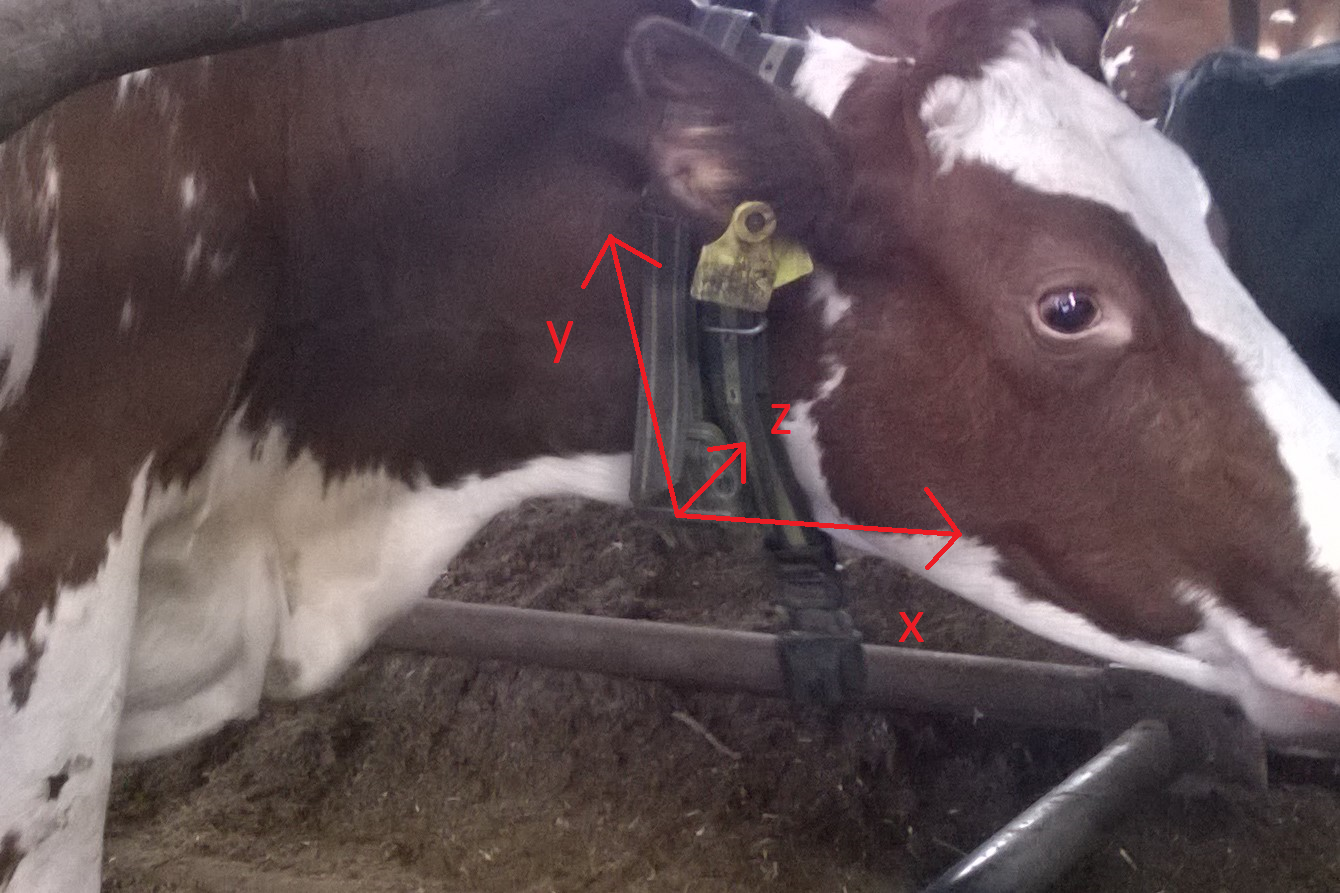
\includegraphics[width = 0.75 \textwidth]{figures/sensorikaulassa1.png}
\caption{Cow wearing a sensor device. The axis directions are illustrated as red arrows in the figure. The sensor is in parallel with a commercial Heatime device shown in this figure.}\label{sensorikaulassakuva}
\end{figure}

\subsection{Data Processing Basics} \label{dataprocessing}

This subsection discusses about the methods used in data analysis. The used methods consists of pure visual observations as well as statistical analysis and more advanced digital signal processing. However, the visual observations remain the primary tool before and after applying any statistical os signal processing method.

\subsubsection{Statistics} \label{statisticssection}

In this study, statistical methods are included in the estrus detection algorithms discussed in section \ref{algorithms}. Furthermore, statistics are used in analysis of duration of SD file operations in section \ref{generalresultssection}.


The statistical methods used in this study are defined as follows \cite{maoltaulukotmatematiikka}:

\begin{itemize}
\item \textit{Mean} is used for describing the most common value of the data set. It is defined as the sum of all values divided the number of values:
\begin{equation} \label{meanequation}
\bar{x} = \frac{\displaystyle \sum\limits^{n}_{i = 1} x(i)}{n}
\end{equation} 

\item \textit{Median} is another number for describing the most common value of the data. In contrast to the mean, it is not that sensitive to exceptionally large or small values. It is defined as the middlemost value of sorted data. If the number of values in the data is even, the median is the sum of two middlemost values divided by two.

\textit{Median} is the middlemost number of the data set sorted from smallest to largest numbers. If the number of elements in array is even, the median is the mean value of the two middlemost values.

\item \textit{Variance} describes the expectation of the squared deviation of a random variable from its mean, and it informally measures how far a set of (random) numbers are spread out from their mean:
\begin{equation} \label{varianceequation}
s^2 = \frac{ \sum\limits_{i = 1}^{n}(x(i) - \bar{x})^2}{n}
\end{equation} 

\item \textit{Standard deviation} describes the amount of variation in the data set. A low standard deviation means the values tend to be close to the mean value, whereas a high value means the values tend to be far from the mean. In contrast to the variance, the standard deviation describes the ``typical''  distance between the values and the mean. The standard deviation is actually the square root of variance:
\begin{equation} \label{standarddeviationequation}
s = \sqrt{\frac{ \sum\limits_{i = 1}^{n}(x(i) - \bar{x})^2}{n}}
\end{equation}

\item \textit{Minimum value} is the smallest value in the data set.

\item \textit{Maximum value} is the largest value in the data set.

\item \textit{Range} is the difference of the minimum and maximum values.
\end{itemize}





\subsubsection{Fourier Transform}

Discrete Fourier transform (DFT) is linear mapping of a signal from time domain to frequency domain \cite{rao2012fast}. That is, a time variant sample can be transformed into frequency domain for providing the frequency spectrum of the data. In this study, the frequency spectrum of cow behavior is valuable information in deciding the the bandwidth of the accelerometer.


\subsubsection{Digital Filters} \label{filters}


The Bosch Sensortec BMA222e accelerometer provides two on chip filters: one 2nd order low-pass filter and another 1st order high-pass filter for offset compensation \cite{bma222datasheet}. Digital filters can be divided into two categories, filters with finite impulse response (FIR) and filters with infinite impulse response (IIR). The main difference between these filters is that the output of a FIR filter is dependent only on the input, whereas, the output of an IIR filter is dependent also on the previous outputs of the filter. Therefore, \cite{digitalfilters} \cite{khan2005digital}.

The digital signal processing methods consists of applying filter and other mathematical methods. In these methods, any features of the sensors could be simulated afterwards instead of using the features of the sensor. E.g., offset compensation using the low pass filter causes the loss in information of orientation of the device.

Filters with infinite impulse response (IIR):



\begin{figure}[htb]
\centering
\begin{tikzpicture}
% Place nodes using a matrix
	\matrix (m1) [row sep=2.5mm, column sep=5mm]
	{		%--------------------------------------------------------------------
		\node[dspnodeopen,dsp/label=above] (m00) {$x[n]$}; &
		\node[coordinate] (m01) {}; &
		\node[dspnodefull] (m02) {}; &
		\node[coordinate] (m03) {}; &
		\node[dspgainr] (m04) {$b_0$}; &
		\node[coordinate] (m05) {}; & 
		\node[dspadder]	(m06) {}; &
		\node[coordinate] (m07) {}; &
		\node[dspnodeopen,dsp/label=above] (m0X) {$y[n]$}; 
		\\
	%--------------------------------------------------------------------
		\node[coordinate] (m10) {}; &
		\node[coordinate] (m11) {}; &
		\node[dspsquare] (m12) {$\z^{-1}$}; &
		\node[coordinate] (m13) {} ; &
		\node[coordinate] (m14) {};          &
		\node[coordinate](m15) {}; &
		\node[coordinate] (m16) {}; &
		\node[coordinate] (m17) {}; &
		\node[coordinate] (m1X) {};         
		\\
	%--------------------------------------------------------------------
		\node[coordinate] (m20) {}; &
		\node[coordinate] (m21) {}; &
		\node[dspnodefull] (m22) {}; &
		\node[coordinate] (m23) {} ; &
		\node[dspgainr] (m24) {$b_1$};          &
		\node[coordinate](m25) {}; &
		\node[dspadder] (m26) {}; &
		\node[coordinate] (m27) {}; &
		\node[coordinate] (m2X) {};         
		\\
	%--------------------------------------------------------------------
		\node[coordinate] (m30) {}; &
		\node[coordinate] (m31) {}; &
		\node[dspsquare] (m32) {$\z^{-1}$}; &
		\node[coordinate] (m33) {} ; &
		\node[coordinate] (m34) {};          &
		\node[coordinate](m35) {}; &
		\node[coordinate] (m36) {}; &
		\node[coordinate] (m37) {}; &
		\node[coordinate] (m3X) {};         
		\\
	%--------------------------------------------------------------------
		\node[coordinate] (m40) {}; &
		\node[coordinate] (m41) {}; &
		\node[dspnodefull] (m42) {}; &
		\node[coordinate] (m43) {}; &
		\node[dspgainr] (m44) {$b_2$}; &
		\node[coordinate] (m45) {}; &
		\node[dspadder] (m46) {}; &
		\node[coordinate] (m47) {}; &
		\node[coordinate] (m4X) {};
		\\
		\\
		\\
		%--------------------------------------------------------------------
		\node[coordinate] (m50) {}; &
		\node[coordinate] (m51) {}; &
		\node[dspsquare] (m52) {$\z^{-1}$}; &
		\node[coordinate] (m53) {} ; &
		\node[coordinate] (m54) {};          &
		\node[coordinate](m55) {}; &
		\node[coordinate] (m56) {}; &
		\node[coordinate] (m57) {}; &
		\node[coordinate] (m5X) {};         
		\\
	%--------------------------------------------------------------------
		\node[coordinate] (m60) {}; &
		\node[coordinate] (m61) {}; &
		\node[coordinate] (m62) {}; &
		\node[coordinate] (m63) {}; &
		\node[dspgainr] (m64) {$b_n$}; &
		\node[coordinate] (m65) {}; &
		\node[coordinate] (m66) {}; &
		\node[coordinate] (m67) {}; &
		\node[coordinate] (m6X) {};
		\\
		%--------------------------------------------------------------------
	};
		
	\draw[dspflow] (m00) -- (m02);
	\draw[dspconn] (m02) -- (m04);
	\draw[dspconn] (m04) -- (m06);
	\draw[dspflow] (m06) -- (m0X);	
	\draw[dspconn] (m02) -- (m12);
	\draw[dspline] (m12) -- (m22);
	\draw[dspconn] (m22) -- (m32);
	\draw[dspline] (m32) -- (m42);	
	\draw[dspconn] (m26) -- (m06);
	\draw[dspconn] (m46) -- (m26);	
	\draw[dspconn] (m22) -- (m24);
	\draw[dspconn] (m24) -- (m26);	
	\draw[dspconn] (m42) -- (m44);
	\draw[dspconn] (m44) -- (m46);	
	\draw[dspconn, dashed] (m42) -- (m52);
	\draw[dspline] (m52) -- (m62);
	\draw[dspconn] (m62) -- (m64);
	\draw[dspline] (m64) -- (m66);
	\draw[dspline] (m66) -- (m56);
	\draw[dspconn, dashed] (m56) -- (m46);

\end{tikzpicture}
\caption{An example of an $n$\textsuperscript{th} order FIR filter}
\end{figure}

\begin{equation}
y[k] = b_0 x[k] + b_1 x[k-1] + b_2 x[k-2] + \dots + b_{n-1} x[k+1-n] + b_n x[k-n]
\end{equation}



\begin{equation}
\begin{aligned}
y[k] = b_0 x[k] + b_1 x[k-1] + b_2 x[k-2] + \dots + b_n x[k-n] \\
-a_1 y[n-1] - a_2 y[n-2] - \dots - a_m y[k-m]
\end{aligned}
\end{equation}


and filter with finite impulse respones (FIR):





\begin{figure}[htb]
\centering
\begin{tikzpicture}
% Place nodes using a matrix
	\matrix (m1) [row sep=2.5mm, column sep=5mm]
	{		%--------------------------------------------------------------------
		\node[dspnodeopen,dsp/label=above] (m00) {$x[n]$}; &
		\node[coordinate] (m01) {}; &
		\node[dspnodefull] (m02) {}; &
		\node[coordinate] (m03) {}; &
		\node[dspgainr] (m04) { $b_0$}; &
		\node[coordinate] (m05) {}; & 
		\node[dspadder]	(m06) {}; &
		\node[coordinate] (m07) {}; &
		\node[dspgainr] (m08) {$1$}; &
		\node[coordinate] (m09) {}; &
		\node[dspnodefull] (m010) {}; &
		\node[coordinate] (m011) {}; &
		\node[dspnodeopen,dsp/label=above] (m0X) {$y[n]$}; 
		\\
	%--------------------------------------------------------------------
		\node[coordinate] (m10) {}; &
		\node[coordinate] (m11) {}; &
		\node[dspsquare] (m12) {$\z^{-1}$}; &
		\node[coordinate] (m13) {}; &
		\node[coordinate] (m14) {}; &
		\node[coordinate] (m15) {}; &
		\node[coordinate] (m16) {}; &
		\node[coordinate] (m17) {}; &
		\node[coordinate] (m18) {}; &
		\node[coordinate] (m19) {}; &
		\node[dspsquare] (m110) {$\z^{-1}$}; &
		\node[coordinate] (m111) {}; &
		\node[coordinate] (m1X) {};         
		\\
	%--------------------------------------------------------------------
		\node[coordinate] (m20) {}; &
		\node[coordinate] (m21) {}; &
		\node[dspnodefull] (m22) {}; &
		\node[coordinate] (m23) {} ; &
		\node[dspgainr] (m24) {$b_1$};          &
		\node[coordinate](m25) {}; &
		\node[dspadder] (m26) {}; &
		\node[coordinate] (m27) {}; &
		\node[dspgainl] (m28) {$-a_1$}; &
		\node[coordinate] (m29) {}; &
		\node[dspnodefull] (m210) {}; &
		\node[coordinate] (m211) {}; &
		\node[coordinate] (m2X) {};         
		\\
	%--------------------------------------------------------------------
		\node[coordinate] (m30) {}; &
		\node[coordinate] (m31) {}; &
		\node[dspsquare] (m32) {$\z^{-1}$}; &
		\node[coordinate] (m33) {} ; &
		\node[coordinate] (m34) {};          &
		\node[coordinate](m35) {}; &
		\node[coordinate] (m36) {}; &
		\node[coordinate] (m37) {}; &
		\node[coordinate] (m38) {}; &
		\node[coordinate] (m39) {}; &
		\node[dspsquare] (m310) {$\z^{-1}$}; &
		\node[coordinate] (m311) {}; &
		\node[coordinate] (m3X) {};         
		\\
	%--------------------------------------------------------------------
		\node[coordinate] (m40) {}; &
		\node[coordinate] (m41) {}; &
		\node[dspnodefull] (m42) {}; &
		\node[coordinate] (m43) {}; &
		\node[dspgainr] (m44) {$b_2$}; &
		\node[coordinate] (m45) {}; &
		\node[dspadder] (m46) {}; &
		\node[coordinate] (m47) {}; &
		\node[dspgainl] (m48) {$-a_2$}; &
		\node[coordinate] (m49) {}; &
		\node[dspnodefull] (m410) {}; &
		\node[coordinate] (m411) {}; &
		\node[coordinate] (m4X) {};
		\\
		\\
		\\
		%--------------------------------------------------------------------
		\node[coordinate] (m50) {}; &
		\node[coordinate] (m51) {}; &
		\node[dspsquare] (m52) {$\z^{-1}$}; &
		\node[coordinate] (m53) {} ; &
		\node[coordinate] (m54) {};          &
		\node[coordinate](m55) {}; &
		\node[coordinate] (m56) {}; &
		\node[coordinate] (m57) {}; &
		\node[coordinate] (m58) {}; &
		\node[coordinate] (m59) {}; &
		\node[dspsquare] (m510) {$\z^{-1}$}; &
		\node[coordinate] (m511) {}; &
		\node[coordinate] (m5X) {};         
		\\
	%--------------------------------------------------------------------
		\node[coordinate] (m60) {}; &
		\node[coordinate] (m61) {}; &
		\node[coordinate] (m62) {}; &
		\node[coordinate] (m63) {}; &
		\node[dspgainr] (m64) {$b_n$}; &
		\node[coordinate] (m65) {}; &
		\node[dspadder] (m66) {}; &
		\node[coordinate] (m67) {}; &
		\node[dspgainl] (m68) {$-a_n$}; &
		\node[coordinate] (m69) {}; &
		\node[coordinate] (m610) {}; &
		\node[coordinate] (m611) {}; &
		\node[coordinate] (m6X) {};
		\\
		%--------------------------------------------------------------------
	};
		
	\draw[dspflow] (m00) -- (m02);
	\draw[dspconn] (m02) -- (m04);
	\draw[dspconn] (m04) -- (m06);
	\draw[dspflow] (m010) -- (m0X);	
	\draw[dspconn] (m06) -- (m08);
	\draw[dspflow] (m08) -- (m010);
	
	\draw[dspconn] (m02) -- (m12);
	\draw[dspline] (m12) -- (m22);
	\draw[dspconn] (m22) -- (m32);
	\draw[dspline] (m32) -- (m42);	
	\draw[dspconn] (m26) -- (m06);
	\draw[dspconn] (m46) -- (m26);	
	\draw[dspconn] (m22) -- (m24);
	\draw[dspconn] (m24) -- (m26);	
	\draw[dspconn] (m42) -- (m44);
	\draw[dspconn] (m44) -- (m46);	
	\draw[dspconn, dashed] (m42) -- (m52);
	\draw[dspline] (m52) -- (m62);
	\draw[dspconn] (m62) -- (m64);
	\draw[dspconn] (m64) -- (m66);
	\draw[dspline] (m66) -- (m56);
	\draw[dspconn, dashed] (m56) -- (m46);
	
	\draw[dspconn] (m010) -- (m110);
	\draw[dspconn] (m68) -- (m66);
	\draw[dspconn] (m48) -- (m46);
	\draw[dspconn] (m28) -- (m26);
	\draw[dspconn] (m210) -- (m28);
	\draw[dspconn] (m410) -- (m48);
	\draw[dspconn] (m610) -- (m68);
	\draw[dspline] (m110) -- (m210);
	\draw[dspconn] (m210) -- (m310);
	\draw[dspline] (m310) -- (m410);
	\draw[dspconn, dashed] (m410) -- (m510);
	\draw[dspline] (m510) -- (m610);
\end{tikzpicture}
\caption{An example of an $n$-th order IIR filter in direct form I}
\end{figure}

\subsubsection{Sliding Window}

In this study, windowing is means analysis and calculus of data in segments instead of entire data set. The windowing method in this study is analogous to windowing in signal processing \cite{tan2007digital,miao2007signal} \dots

\subsection{Etrus Detection Algorithms} \label{algorithms}

This section introduces a fundamental concept for the detection of  a dairy cow. In general, the cow behavior changes along with the phases of estrus the cycle \ref{estruscycle}. That is, the activity level increases in proestrus 

That is, the cow becomes exceptionally active in proestrus, whereas the activity normalizes in estrus. Therefore, 

This subsection discusses about plausible algorithms for dairy cow estrus detection. The algorithms consists of methods of data analysis described foregoing subsections. In fact, algorithms are sequences of methods that provide answer to the question whether the cow is in estrus or not.

The principle idea of estrus detection is based on high pro-estrus activity of the cow. That is, the cow attends to move significantly more than usually. Furthermore, the time spent on rumination degrades meanwhile. Thus, it is considered to detect the pro-estrus instead of the actual estrus. Additionally, it is beneficial since, it provides wider time window for insemination. In conclusion, the basis of the algorithm is defining the amount of activity.

Considering the activity measurement in wearable devices for people, the activity is typically measured as sum of absolute values of all the axis. In studies, it has been proved it to match to the real energy consumption better than the absolute value.

Windowed mean value:

\begin{equation}
\bar{x}(k) = \frac{ \sum\limits^{k}_{i = k - n} x(i)}{n}
\end{equation}, where $n$ is the size of the window.


The main features of all the following algorithms are as follows:
\begin{enumerate}

\item \textbf{Process data} --- Data processing consists of algorithm specific data functions. These functions may include data filtering and other computations. These functions are discussed in detail in the following subsections. All the remaining phases of the algorithms follows the same pattern discussed below.

\item \textbf{Sum results} --- The results of data processing are summed within time windows. The length of the time window should approximate the duration of the proestrus. Additionally, these time windows shall overlap in order to provide more continuous impression of ongoing state of estrus cycle. Furthermore, excessively long time windows without overlapping could delay the detection of the estrus. Thus, cause the failure of insemination as a consequence.

\begin{equation}
u(k) =\sum\limits^{nk}_{i = nk - m} x(i) \mathrm{\hspace{1em}, where}
\end{equation}
$k$ is the index of summed results, $n$ is an incremental step size and $m$ is the size of the time window.

\item \textbf{Remove offset} --- The resulting data after summing may differ significantly within algorithm depending on the parameters as well as between the algorithms. Therefore, any existing offset in the data should be removed. This means adjusting the data so that the normal behavior appears around the zero. The median of the data describes the amount of the offset more reliable than mean value. Hence, median is less sensitive to proestrus peaks in the data.  

\begin{equation}
u(k) = x(k) - \tilde{x} \mathrm{\hspace{1em}, where}
\end{equation}
$\tilde{x}$ is the median value of $x$.

\item \textbf{Normalize} --- After removing the offset, the data shall be normalized. In this case, the normalizing means scaling the data so that no extreme value shall exceed the range of from $-1$ to $1$.

\begin{equation}
u(k) = \frac{x(k)}{\max  \left| x \right|} 
\end{equation}


\item \textbf{Threshold} --- Finally, thresholds are used for indicating the beginning and the end of the proestrus. That is, exceeding the first threshold indicates the beginning of the proestrus and next, the going below indicates the end of the proestrus. The thresholds for deciding whether the cow is in estrus or not should be separate. The end of proestrus signals to the cattle tender to prepare for insemination. The principle of the proestrus detection is presented in the following pseudo code. 

\Clanguage
\begin{lstlisting}
for (i = 0 ; i < length(x); i ++)
 if (x(i) > threshold1 && proestrus == false)	
  proestrus = true;
 else if (x(i) < threshold && proestrus == true)
  proestrus = false;	
\end{lstlisting}
Additionally, each change of the estrus state should trigger an alert.


\end{enumerate}


\subsubsection{Activity Measurement}

The concept of the first estrus detection algorithm is analogous to an accelerometer based estimation of total energy consumption \cite{Kang2012}. However, finding of any correlation between the activity and the energy consumption is not a focus of this study. Nevertheless, this algorithm utilizes the same method for determination of the cow activity level. 


The first algorithm is based on pure analysis of full the data set. The algorithm is analogous to an estimation of energy consumption using accelerometers   \dots



\begin{enumerate}
\item \textbf{Filter} --- Hence, the 

\begin{equation}
y(k) = a_0 x(k) + a_1 x(k-1) + a_2 x(k-2) - b_1 y(k-1) - b_2 y(k-2)
\end{equation}

\item \textbf{Compute} --- The actual core of this algorithm is the length of the acceleration vector and it is defined as \begin{equation}
u(i) = \sqrt{x^2(i) + y^2(i) + z^2(i)} 
\end{equation}

\end{enumerate}


\subsubsection{Variance Detection}

The first algorithm had a basis in continuous computation of continuous data stream. In contrast to the first algorithm, the second algorithm attempts to reduce the amount of required data. That is, using standard data samples in regular intervals instead of continuous stream. Furthermore, the calculus of the algorithms are different. The ground of the first algorithm was in summing of the lengths of the total acceleration vectors, whereas this algorithms attempts to determinate the level of variance 


The first algorithm calculated the length of the total acceleration vectors. Thus, estimated the energy consumption. Alternatively, this second algorithm detects the level of variation in the acceleration data rather than the total amount of movement.

Originally, the concept of a variance based algorithm arose along with the analysis of the recorded data sets. 


%Originally, the concept of a variance based algorithm arose among the analysis of the first recorded data set. The data consisted of two distinct period. They differed in variance as well as in offset. In theory, both of these differences could have been used as a basis of an algorithm. However, the reliability of the offset is questionable, hence the pose of the device is not strictly fixed in the neck of a cow. Additionally, offset based algorithm would prevent the use of the offset compensation of the accelerometer. Consequently, it would set unnecessary restrictions for future development. Moreover, the difference in offset was mostly significant in the x-axis data. Conversely, the amount of variance appeared evenly on each axis. Furthermore, variance is offset independent. Thus, variance based algorithm does not require any high-pass filtering before data processing. 

\begin{enumerate}

\item \textbf{Get a sample} --- In this algorithm, the data is processed in samples instead of data stream. 

\item \textbf{Compute Variance} --- Compute the variance of the sample

\begin{equation} \label{samplevariance}
u_x(k) = \frac{\sum \limits_{i=nk-m}^{nk} (x(i) - \bar{x})^2}{m} \mathrm{\hspace{1em}, where}
\end{equation}
$m$ is the size of the data sample, $n$ is the distance between the samples and $k$ is the index of the output data. 

\begin{equation}
u_{tot} = u_x + u_y + u_z
\end{equation}

\end{enumerate}


\subsubsection{Inactivity Detection}

The first two algorithms were based on relatively demanding computations considering micro-controller (MCU) environments. The first algorithm required a continuous data stream and calculating powers of two and square roots. The second algorithm did not require a continuous data stream. However, the algorithm included computing of variance which includes sum, square root and power of two as discussed in section \ref{statisticssection}. Furthermore, the available dynamic memory of micro-controllers are restricted. Therefore, it limits the maximum number of retained data points for computing the variance. In contrast, the third algorithm attempts to reduce the computation in the MCU. Therefore, it requires more advanced deployment of the features of the accelerometer. Accordingly, an interrupt driven approach becomes sensible. That is, the the MCU only counts the number of interrupt events whereas, the accelerometer performs all other computations.

In addition to transferring most of the calculus from MCU to accelerometer, the logic itself could be inverted. That is, monitoring inactivity instead of activity. For this perspective, the accelerometer provides the feature of \textit{no motion detection} which was discussed in section \ref{hardwaresection}. This feature suits fairly well to the aspect of transferring the computation from MCU to micro-controller and observing inactivity instead of activity. However, this study bases on recorded data instead of testing these configurations real animals. Therefore, the algorithm described below is purely a simulation of the features of the accelerometer. In consequence, the results achieved in this study might differ from those of real life.

This inactivity detection algorithm complies with the algorithm structure discussed earlier in this section. The data processing phase of this algorithm is as follows.

\begin{enumerate}
\item \textbf{Get Slope} --- The slope is the acceleration difference. That is, the previous value subtracted from the current value: 

\begin{equation}
u[i] = x[i] - x[i-1]
\end{equation}

Furthermore, the slope is offset independent. Hence, the slope is actually first order FIR filter with infinite attenuation at zero frequency, sampling frequency and its harmonics.

\item \textbf{Detect inactivity} --- According to the specifications of the accelerometer, a no-motion interrupt is triggered if the absolute value of the slope remains below of a preset threshold for a preset duration of time. The following pseudo code represents the software implementation for the no-motion detection. 

\Clanguage
\begin{lstlisting}
for (i = 0 ; i < length(x); i ++)
 if (x(i) > threshold)	
  prev_i = i;
 if (i - prev_i > passivity_period)
  passivity(i) = 1;
  prev_i = 1;	
\end{lstlisting}

In this study, the passivity array has the same length as the acceleration data array and it is initialized as zeros. During the execution, the algorithm processes through the entire data set. Meanwhile, any occurred no-motion condition yields the value of one into the passivity array. In consequence, the resulting passivity array consists mostly of zeros and few of ones within. Furthermore, the indexes of the ones are directly related to the time of the occurrence. Thus, it enables concluding the level of inactivity in certain range of time. 

\end{enumerate}

Next, after these two specific phases of data processing phases the algorithm proceeds its normal sequence as discussed earlier in this section. 


\clearpage

\section{Results} \label{resultssection}
 
This section surveys through the results of the data recording processes. As described in section \ref{datarecordingprocess}, the data was recorder on two separate occasions



\subsection{General Review} \label{generalresultssection}

This subsection discusses about rather general results whereas the scope of subsection \ref{estrusdetectionsection} is in the detection of estrus. In despite of the general nature of these results, they are advantageous considering research in future. Furthermore, some early stage results such as the frequency analysis discussed later in this section were used for improving the sensor device software. This subsection covers the frequency analysis of the first recorder data set as well as statistical analysis of the acceleration data and some interesting features of SD file operations.

\subsubsection{First Data Set}

Arvoidaan ensimmäisen datasetin tuloksia, mutta myös hardwarea ja software. Jotain johtopäätöksiä


\subsubsection*{Frequency Spectrum}

The frequency spectrum of the first recorded data was analyzed using Fast Fourier Transform (FFT) as discussed in section \ref{signalprocessingsection}. The Fourier Transform was applied on the raw data without any other signal processing methods such as offset compensation. Therefore, the frequency spectrum of each axis consists of significant components at zero frequency and nearby. These components could have been reduced using such offset compensation as a high-pass filter discussed in section \ref{hardwaresection}. However, applying offset compensation to the data does not provide any additional information in frequency domain. Thus, awareness of the offset component is enough considering the usage of the results. The results of the FFT are represented in figure \ref{frequenyspectrumfigure}.

\begin{figure}[htb]
\centering
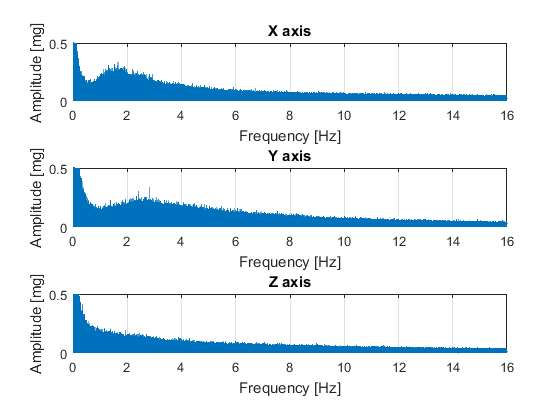
\includegraphics[width = 0.75\textwidth]{figures/frequencyanalysis2.png}
\caption{The results of the frequency analysis of the first data set. The frequency spectrum of each axis consists of significant components at frequencies close to zero-frequency and minor components at non-zero frequencies.} \label{frequenyspectrumfigure}
\end{figure}



\subsubsection*{SD File Operations}

In the first data recording process, it was desired to record the data in as high bandwidth as possible. The maximum bandwidth of the accelerometer were \SI{1000}{\hertz}. Consequently, the update time was \SI{0.5}{\milli \second}. However, the duration of SD file operations restricts the maximum recording bandwidth significantly. Finally, in the first data recording process the bandwidth was selected to be \SI{125}{\hertz}. Yet, the file operations exceeded the time ...

SD card file operation times were recorded after the actual data recording using the original hardware. The original software was improved with timer operations in order to enable the recording of the file operation times. The file operation times had an affect on the data recording process. The time consumed for opening a file increased among the file size. The minimum opening time was \SI{7.26}{\milli\second} and the maximum time for \SI{1.37}{\giga \byte} file a was \SI{1440}{\milli \second}. The average value was \SI{747.14}{\milli \second}. The file closing times varied from \SI{8.04}{\milli \second} to \SI{160.03}{\milli \second} and seemed not to be dependent on the file size. The average file closing time was \SI{19.75}{\milli \second}. The time spent of writing a single data line was from \SI{56}{\micro \second} to \SI{162.36}{\milli\second} and the average was \SI{997.76}{\milli\second}.

\begin{table} \caption{File operation times of the first data recording hardware and software}
\centering
\begin{tabular}{| l | l | l | l | l |}
\hline
Operation & Min [\SI{}{\milli \second}] & Max [\SI{}{\milli \second}] & Mean [\SI{}{\milli \second}]& Variance [\SI{}{\milli \second}]\\ \hline
Open file & 2 & 3 & 4 & 5 \\ \hline
Close file &  &  &  &  \\ \hline
Write line &  &  &  &  \\ \hline
\end{tabular}
\end{table}

\subsubsection{Second Data Set}

ARvioidaan toisen (ja kolmannen) datasetin tuloksia, mutta myös laitteistoa ja ohjelmistoa. Jotain johtopäätöksiä.



This subsection concentrates in the results of estrus detection. As discussed in section \ref{datarecordingprocess} six cows were used in data recording process. However, two out of six data recordings failed. Thus, that data had to be discarded. The estruses were confirmed by Heatime estrus detection system.


In this study, a total of six cows were used for long period data recording.

\begin{figure}[htb]
\centering
\includegraphics[width = 0.75\textwidth]{figures/punainenkiima}
\caption{The estrus of the cow marked with red and green color. This cow had two estruses during the data recording period.}
\label{punainenkiimaheattime}
\end{figure}



\subsection{Algorithm Evaluation}

\subsubsection{Activity Measurement}

\subsubsection{Variance Detection}

\subsubsection{Inactivity Detection}



The first set of data provided relatively wide frequency spectrum of data.



The sampling period provided a total of three probable estruses. One of the sensors failed during the sampling period, and therefore, no estrus could be estimated. However, one of the cows had two estruses during the sampling period and thus, compensated the failed sensor.

Based on pure visual analysis of the acceleration data, the red cow has two highly active proestrus periods. First begins December the 22nd at 9 pm end ends December the 23rd at 9 am. The second period begins January the 4th at 2 am and ends 6 pm. Proper insemination is from 6 to 24 hours after proestrus period.

The estrus was detected using Heatime estrus detection system. The detected estruses are represented in figures...

%\begin{figure}[htb]
%\centering
%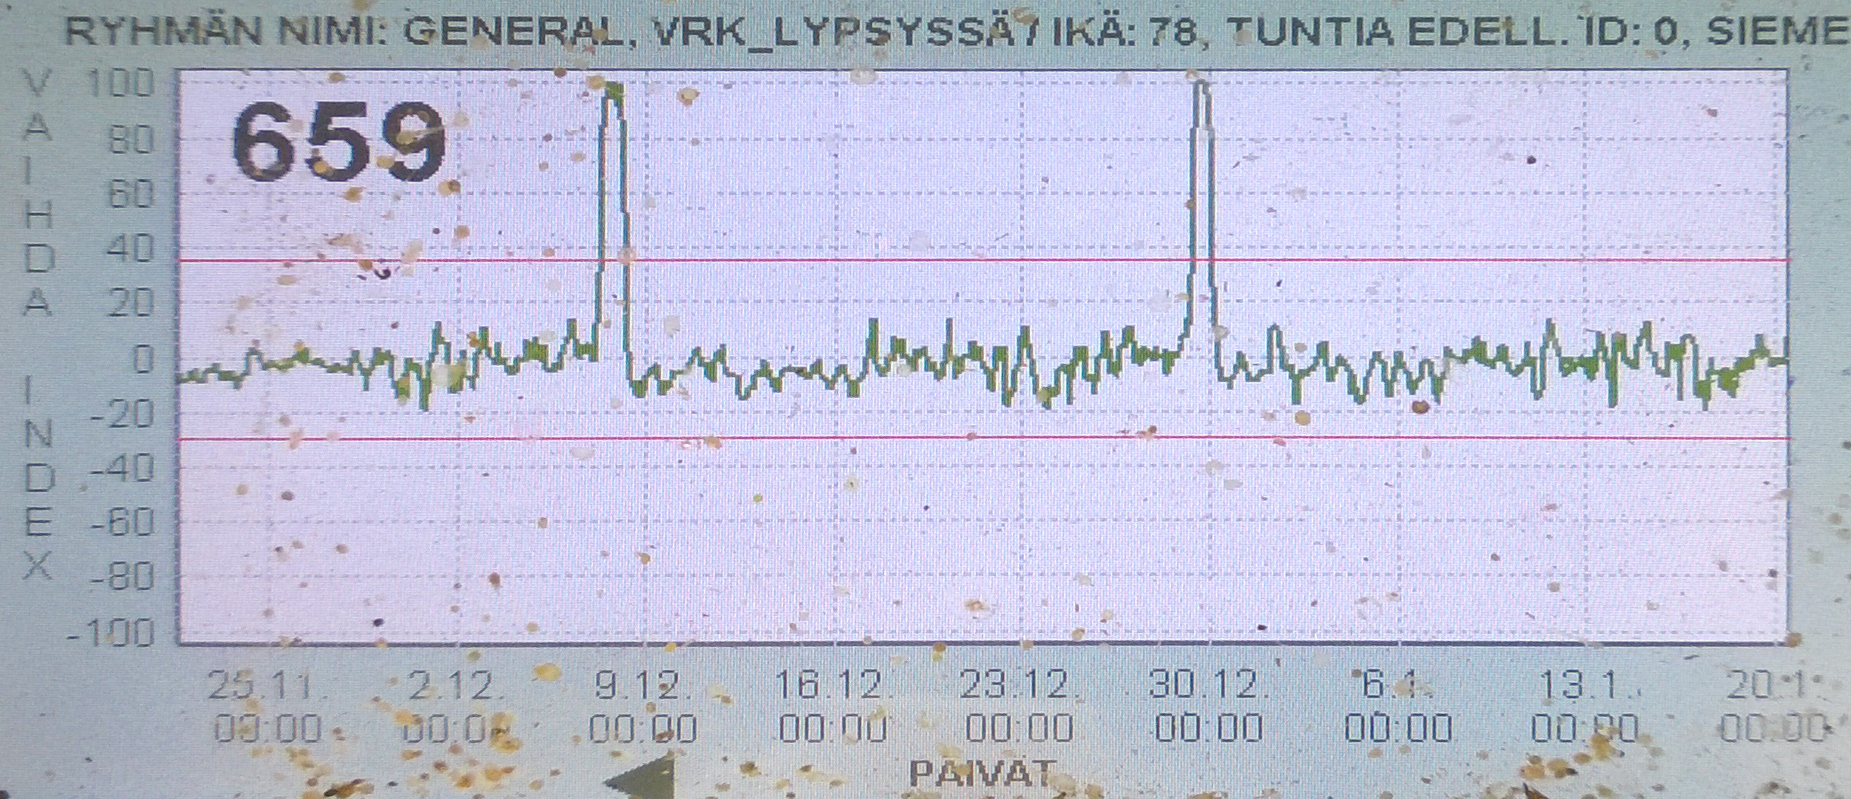
\includegraphics[width = 0.75\textwidth]{figures/sininenkiima.png}
%\caption{The estrus of the cow marked with blue color. However, the data recording stopped before proestrus activity, end therefore, estrus could not be detected using the recorded data.} \label{sininenkiimaheattime}
%\end{figure}
%
%\begin{figure}[htb]
%\centering
%\includegraphics[width = 0.75\textwidth]{figures/keltainenkiima.png}
%\caption{The estrus of the cow marked with yellow color. The latter estrus of this figure was timed during the data recording and, therefore, it could be detected by the data. The red line represents the cow activity and the green line represents the ruminating time.}
%\label{keltainenkiimaheattime}
%\end{figure}



\begin{figure}[htb]
\centering
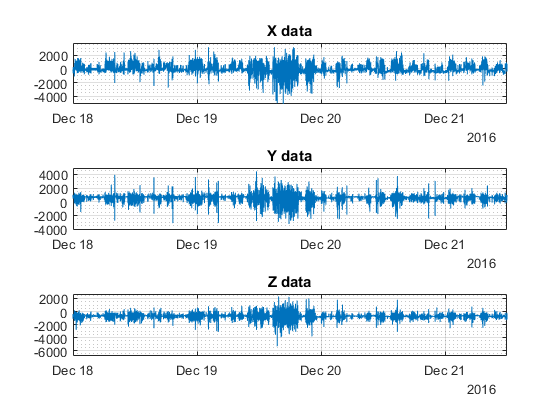
\includegraphics[width = 0.75\textwidth]{figures/keltainenkiimadata.png}
\caption{The estrus behaviour in recoreded data of the yellow cow.}
\label{keltainenkiimadata}
\end{figure}

\begin{figure}[htb]
\centering
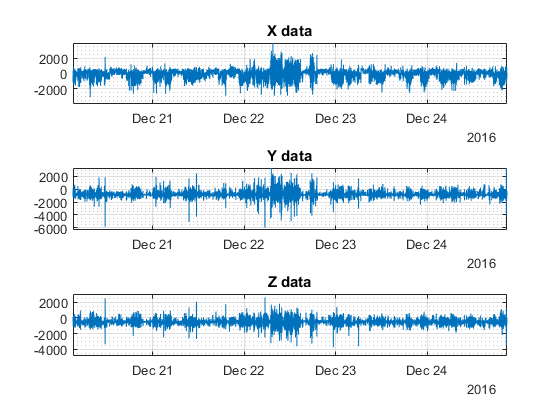
\includegraphics[width = 0.75\textwidth]{figures/punainenkiimadata1.png}
\caption{The first estrus activity period in the recorded data of the red cow.}
\label{punainenkiimadata1}
\end{figure}

\begin{figure}[htb]
\centering
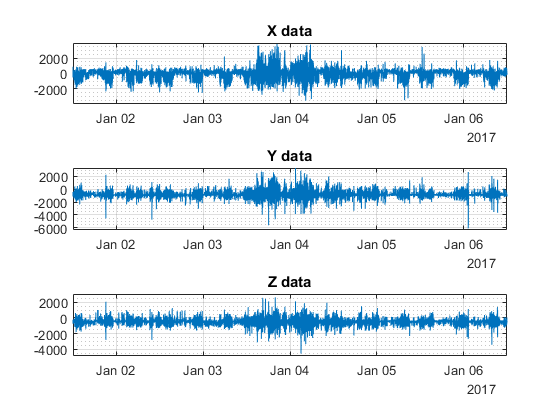
\includegraphics[width = 0.75\textwidth]{figures/punainenkiimadata2.png}
\caption{The second activity period of the red cow.}
\label{punainenkiimadata2}
\end{figure}



The activity could be measured in several ways. Pedometers measures the number of steps. However, sensor worn in neck could not probably be used for step counting and therefore, no steps were estimated. Human activity bracelets and other devices could measure steps but if total energy consumption is being estimated, the values of acceleration should be taken into account. A research have shown that the sum of absolute value of the axis, instead of a absolute value is the best simple estimate for energy consumption and therefore, a good activity measure.

The cow activity was measured as a sum of absolute value acceleration vector. The activity was summed over a varying time window from 6 hours to 36 six hours. Since the resulting activity is always a sum of past activity, this method causes delay and widening of the activity peak. However, the size of the window does not affect the steepness of the rising or falling edges. Nevertheless, the size of the window widens the peaks if the window size is too high. In result, increasing the window might delay the oestrus detection, if the detection has dependencies in the falling edge. Based on the three found heat activity peaks of oestrus, an optimal window size is somewhere between 9 end 12 hours.

\begin{figure}[htb]
\centering
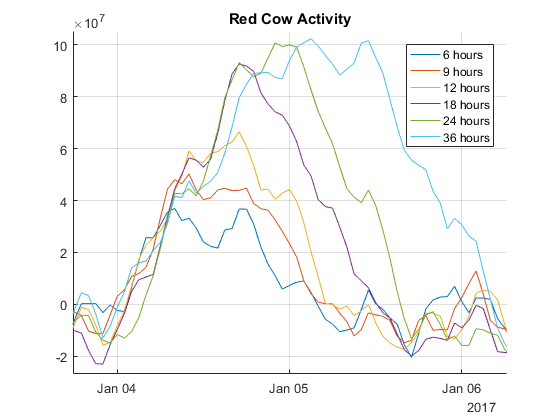
\includegraphics[width = 0.75\textwidth]{figures/redcowactivity2.png}
\caption{The activity curves of a cow in estrus. The width of the window varies. The optimal window size is approximately between form 9 to 12 hours.}
\end{figure}

\subsection{Conclusions}



\clearpage

\section{Summary} 


Summary of all the previous. Alternatively ``Discussion'' or ``Conclusions''...


\clearpage
%% Lähdeluettelo

\thesisbibliography

%\begin{thebibliography}{99}

\begin{thebibliography}{99}

\begin{thebibliography}{99}

\include{bibliography.tex}

%% Alla pilkun jälkeen on pakotettu oikea väli \<välilyönti>-merkeillä.
\bibitem{Kauranen} Kauranen,\ I., Mustakallio,\ M. ja Palmgren,\ V.
  \textit{Tutkimusraportin kirjoittamisen opas opinnäytetyön
    tekijöille.}  Espoo, Teknillinen korkeakoulu, 2006.

\bibitem{Itkonen} Itkonen,\ M. \textit{Typografian käsikirja.} 3.\
  painos.  Helsinki, RPS-yhtiöt, 2007.

\bibitem{Koblitz} Koblitz,\ N. \textit{A Course in Number Theory and
    Cryptography. Graduate Texts in Mathematics 114.}  2.\ painos. New
  York, Springer, 1994.

%% Kun on useampi nimikirjain, jokaisen nimikirjaimen väliin
%% kuuluu välilyönti. Oikea välin määrä on saatu \<välilyönnillä>
\bibitem{bcs} Bardeen,\ J., Cooper,\ L.\ N. ja Schrieffer,\ J.\ R.
  Theory of Superconductivity. \textit{Physical Review,} 1957, vol.\
  108, nro~5, s.\ 1175--1204.

\bibitem{Deschamps} Deschamps,\ G.\ A. Electromagnetics and
  Differential Forms. \textit{Proceedings of the IEEE,} 1981, vol.\
  69, nro~6, s.\ 676--696.

%% Alla esimerkki englanninkielisen tavuttamisen pakottamisesta.
%% Oletusarvoisesti käytetään suomalaista tavutusta, mutta viitteissä
%% esiintyy usein muunkielisiä lauseita, jotka tulevat siten tavutetuksi
%% suomen kielen sääntöjen mukaan. Tämän voi korjata \foreignlanguage-
%% komennolla, jonka ensimmäinen parametri on vieraan kielen nimi ja toinen 
%% on vieraalla kielellä tavutettava teksti. 
\bibitem{Sihvola} Sihvola,\ A.\ et al.
  \foreignlanguage{english}{Interpretation of measurements of helix 
    and bihelix superchiral structures.}
  Teoksessa: Jacob,\ A.\ F. ja
  Reinert,\ J. (toim.) \textit{Bianisotropics '98 7th International
    Conference on Complex Media.}  Braunschweig, 3.--6.6.1998.
  Braunscweig, Technische Universität Braunschweig, 1998, s.\
  317--320.

%% Alla on suomalainen yhdistelmäsukunimi. Sen nimien välissä 
%% käytetään yhdysmerkkiä l. tavuviivaa, kirjoitetaan -.
\bibitem{Lindblom} Lindblom-Ylänne,\ S. ja Wager,\ M.  Tieteellisten
  opinnäytetöiden ohjaaminen. Teoksessa: Lindblom-Ylänne,\ S. ja
  Nevgi,\ A. (toim.) \textit{Yliopisto- ja korkeakouluopettajan
    käsikirja.}  Helsinki, WSOY, 2004, s.\ 314--325.
 
\bibitem{Miinusmaa} Miinusmaa,\ H. Neliskulmaisen reiän poraamisesta
  kolmikulmaisella poralla. Diplomityö, Teknillinen korkeakoulu,
  konetekniikan osasto, Espoo, 1977.

%% Tässä taas pakotettu englanninkielinen tavutus. 
%% Pedanttinen kirjoittaja pakottaa tietysti jokaiseen englanninkieliseen
%% lauseeseen englannin tavutuksen, mutta tässä esityksessä ei näin ole
%% tehty selvyyden ja lähdekoodin luettavuuden takia. 
\bibitem{Loh} Loh,\ N.\ C. High-Resolution Micromachined
  Interferometric Accelerometer. Master's Thesis, Massachusetts
  Institute of Technology, Cambridge,
  \foreignlanguage{english}{Massachusetts,} 1992.

\bibitem{Lonnqvist} Lönnqvist,\ A.
  \foreignlanguage{english}{Applications of hologram-based compact
    range: antenna radiation pattern, radar cross section, and
    absorber reflectivity measurements.}
  Väitöskirja, Teknillinen korkeakoulu, sähkö- ja tietoliikennetekniikan
  osasto, 2006.

\bibitem{sfs} SFS 5342. Kirjallisuusviitteiden laatiminen. 2.\ painos.
  Helsinki, Suomen standardisoimisliitto, 2004. 20~s.

\bibitem{haastattelu} Palmgren,\ V. Suunnittelija. Teknillinen
  korkeakoulu, kirjasto. Otaniementie 9, 02150 Espoo. Haastattelu
  15.1.2007.

\bibitem{Ribeiro} Ribeiro,\ C.\ B., Ollila,\ E. ja Koivunen,\ V.
  \foreignlanguage{english}{Stochastic Maximum-Likelihood Method for
    MIMO Propagation Parameter Estimation.}
 \textit{IEEE Transactions
    on Signal Processing,} verkkolehti, vol.\ 55, nro~1, s.\ 46--55.
  Viitattu 19.1.2007. Lehti ilmestyy myös painettuna. DOI:
  10.1109/TSP.2006.882057.

\bibitem{Stieber} Stieber,\ T. GnuPG Hacks. \textit{Linux Journal,}
  verkkolehti, 2006, maaliskuu, nro~143. Viitattu 19.1.2007. Lehti
  ilmestyy myös painettuna. Saatavissa:
  \url{http://www.linuxjournal.com/article/8732.}

\bibitem{kone} Pohjois-Koivisto,\ T. Voiko kone tulevaisuudessa arvata
  tahtosi?  \textit{Apropos,} verkkolehti, helmikuu, nro~1, 2005.
  Viitattu 19.1.2007.  Saatavissa:
  \url{http://www.apropos.fi/1-2005/prima.php.}

\bibitem{Adida} Adida,\ B.  Advances in Cryptographic Voting Systems.
  Verkkodokumentti. Ph.D.\ Thesis, Massachusetts Institute of
  Technology, Cambridge, 
  \foreignlanguage{english}{Massachusetts,}
  2006. Viitattu 19.1.2007.  Saatavissa:
  \url{http://crypto.csail.mit.edu/~cis/theses/adida-phd.pdf.}

\bibitem{viittaaminen} Kilpeläinen,\ P. WWW-lähteisiin viittaaminen
  tutkielmatekstissä. Verkkodokumentti. Päivitetty 26.11.2001.
  Viitattu 19.1.2007. Saatavissa:
  \url{http://www.cs.uku.fi/~kilpelai/wwwlahteet.html.}

\end{thebibliography}

%% Alla pilkun jälkeen on pakotettu oikea väli \<välilyönti>-merkeillä.
\bibitem{Kauranen} Kauranen,\ I., Mustakallio,\ M. ja Palmgren,\ V.
  \textit{Tutkimusraportin kirjoittamisen opas opinnäytetyön
    tekijöille.}  Espoo, Teknillinen korkeakoulu, 2006.

\bibitem{Itkonen} Itkonen,\ M. \textit{Typografian käsikirja.} 3.\
  painos.  Helsinki, RPS-yhtiöt, 2007.

\bibitem{Koblitz} Koblitz,\ N. \textit{A Course in Number Theory and
    Cryptography. Graduate Texts in Mathematics 114.}  2.\ painos. New
  York, Springer, 1994.

%% Kun on useampi nimikirjain, jokaisen nimikirjaimen väliin
%% kuuluu välilyönti. Oikea välin määrä on saatu \<välilyönnillä>
\bibitem{bcs} Bardeen,\ J., Cooper,\ L.\ N. ja Schrieffer,\ J.\ R.
  Theory of Superconductivity. \textit{Physical Review,} 1957, vol.\
  108, nro~5, s.\ 1175--1204.

\bibitem{Deschamps} Deschamps,\ G.\ A. Electromagnetics and
  Differential Forms. \textit{Proceedings of the IEEE,} 1981, vol.\
  69, nro~6, s.\ 676--696.

%% Alla esimerkki englanninkielisen tavuttamisen pakottamisesta.
%% Oletusarvoisesti käytetään suomalaista tavutusta, mutta viitteissä
%% esiintyy usein muunkielisiä lauseita, jotka tulevat siten tavutetuksi
%% suomen kielen sääntöjen mukaan. Tämän voi korjata \foreignlanguage-
%% komennolla, jonka ensimmäinen parametri on vieraan kielen nimi ja toinen 
%% on vieraalla kielellä tavutettava teksti. 
\bibitem{Sihvola} Sihvola,\ A.\ et al.
  \foreignlanguage{english}{Interpretation of measurements of helix 
    and bihelix superchiral structures.}
  Teoksessa: Jacob,\ A.\ F. ja
  Reinert,\ J. (toim.) \textit{Bianisotropics '98 7th International
    Conference on Complex Media.}  Braunschweig, 3.--6.6.1998.
  Braunscweig, Technische Universität Braunschweig, 1998, s.\
  317--320.

%% Alla on suomalainen yhdistelmäsukunimi. Sen nimien välissä 
%% käytetään yhdysmerkkiä l. tavuviivaa, kirjoitetaan -.
\bibitem{Lindblom} Lindblom-Ylänne,\ S. ja Wager,\ M.  Tieteellisten
  opinnäytetöiden ohjaaminen. Teoksessa: Lindblom-Ylänne,\ S. ja
  Nevgi,\ A. (toim.) \textit{Yliopisto- ja korkeakouluopettajan
    käsikirja.}  Helsinki, WSOY, 2004, s.\ 314--325.
 
\bibitem{Miinusmaa} Miinusmaa,\ H. Neliskulmaisen reiän poraamisesta
  kolmikulmaisella poralla. Diplomityö, Teknillinen korkeakoulu,
  konetekniikan osasto, Espoo, 1977.

%% Tässä taas pakotettu englanninkielinen tavutus. 
%% Pedanttinen kirjoittaja pakottaa tietysti jokaiseen englanninkieliseen
%% lauseeseen englannin tavutuksen, mutta tässä esityksessä ei näin ole
%% tehty selvyyden ja lähdekoodin luettavuuden takia. 
\bibitem{Loh} Loh,\ N.\ C. High-Resolution Micromachined
  Interferometric Accelerometer. Master's Thesis, Massachusetts
  Institute of Technology, Cambridge,
  \foreignlanguage{english}{Massachusetts,} 1992.

\bibitem{Lonnqvist} Lönnqvist,\ A.
  \foreignlanguage{english}{Applications of hologram-based compact
    range: antenna radiation pattern, radar cross section, and
    absorber reflectivity measurements.}
  Väitöskirja, Teknillinen korkeakoulu, sähkö- ja tietoliikennetekniikan
  osasto, 2006.

\bibitem{sfs} SFS 5342. Kirjallisuusviitteiden laatiminen. 2.\ painos.
  Helsinki, Suomen standardisoimisliitto, 2004. 20~s.

\bibitem{haastattelu} Palmgren,\ V. Suunnittelija. Teknillinen
  korkeakoulu, kirjasto. Otaniementie 9, 02150 Espoo. Haastattelu
  15.1.2007.

\bibitem{Ribeiro} Ribeiro,\ C.\ B., Ollila,\ E. ja Koivunen,\ V.
  \foreignlanguage{english}{Stochastic Maximum-Likelihood Method for
    MIMO Propagation Parameter Estimation.}
 \textit{IEEE Transactions
    on Signal Processing,} verkkolehti, vol.\ 55, nro~1, s.\ 46--55.
  Viitattu 19.1.2007. Lehti ilmestyy myös painettuna. DOI:
  10.1109/TSP.2006.882057.

\bibitem{Stieber} Stieber,\ T. GnuPG Hacks. \textit{Linux Journal,}
  verkkolehti, 2006, maaliskuu, nro~143. Viitattu 19.1.2007. Lehti
  ilmestyy myös painettuna. Saatavissa:
  \url{http://www.linuxjournal.com/article/8732.}

\bibitem{kone} Pohjois-Koivisto,\ T. Voiko kone tulevaisuudessa arvata
  tahtosi?  \textit{Apropos,} verkkolehti, helmikuu, nro~1, 2005.
  Viitattu 19.1.2007.  Saatavissa:
  \url{http://www.apropos.fi/1-2005/prima.php.}

\bibitem{Adida} Adida,\ B.  Advances in Cryptographic Voting Systems.
  Verkkodokumentti. Ph.D.\ Thesis, Massachusetts Institute of
  Technology, Cambridge, 
  \foreignlanguage{english}{Massachusetts,}
  2006. Viitattu 19.1.2007.  Saatavissa:
  \url{http://crypto.csail.mit.edu/~cis/theses/adida-phd.pdf.}

\bibitem{viittaaminen} Kilpeläinen,\ P. WWW-lähteisiin viittaaminen
  tutkielmatekstissä. Verkkodokumentti. Päivitetty 26.11.2001.
  Viitattu 19.1.2007. Saatavissa:
  \url{http://www.cs.uku.fi/~kilpelai/wwwlahteet.html.}

\end{thebibliography}

%% Alla pilkun jälkeen on pakotettu oikea väli \<välilyönti>-merkeillä.
\bibitem{Kauranen} Kauranen,\ I., Mustakallio,\ M. ja Palmgren,\ V.
  \textit{Tutkimusraportin kirjoittamisen opas opinnäytetyön
    tekijöille.}  Espoo, Teknillinen korkeakoulu, 2006.

\bibitem{Itkonen} Itkonen,\ M. \textit{Typografian käsikirja.} 3.\
  painos.  Helsinki, RPS-yhtiöt, 2007.

\bibitem{Koblitz} Koblitz,\ N. \textit{A Course in Number Theory and
    Cryptography. Graduate Texts in Mathematics 114.}  2.\ painos. New
  York, Springer, 1994.

%% Kun on useampi nimikirjain, jokaisen nimikirjaimen väliin
%% kuuluu välilyönti. Oikea välin määrä on saatu \<välilyönnillä>
\bibitem{bcs} Bardeen,\ J., Cooper,\ L.\ N. ja Schrieffer,\ J.\ R.
  Theory of Superconductivity. \textit{Physical Review,} 1957, vol.\
  108, nro~5, s.\ 1175--1204.

\bibitem{Deschamps} Deschamps,\ G.\ A. Electromagnetics and
  Differential Forms. \textit{Proceedings of the IEEE,} 1981, vol.\
  69, nro~6, s.\ 676--696.

%% Alla esimerkki englanninkielisen tavuttamisen pakottamisesta.
%% Oletusarvoisesti käytetään suomalaista tavutusta, mutta viitteissä
%% esiintyy usein muunkielisiä lauseita, jotka tulevat siten tavutetuksi
%% suomen kielen sääntöjen mukaan. Tämän voi korjata \foreignlanguage-
%% komennolla, jonka ensimmäinen parametri on vieraan kielen nimi ja toinen 
%% on vieraalla kielellä tavutettava teksti. 
\bibitem{Sihvola} Sihvola,\ A.\ et al.
  \foreignlanguage{english}{Interpretation of measurements of helix 
    and bihelix superchiral structures.}
  Teoksessa: Jacob,\ A.\ F. ja
  Reinert,\ J. (toim.) \textit{Bianisotropics '98 7th International
    Conference on Complex Media.}  Braunschweig, 3.--6.6.1998.
  Braunscweig, Technische Universität Braunschweig, 1998, s.\
  317--320.

%% Alla on suomalainen yhdistelmäsukunimi. Sen nimien välissä 
%% käytetään yhdysmerkkiä l. tavuviivaa, kirjoitetaan -.
\bibitem{Lindblom} Lindblom-Ylänne,\ S. ja Wager,\ M.  Tieteellisten
  opinnäytetöiden ohjaaminen. Teoksessa: Lindblom-Ylänne,\ S. ja
  Nevgi,\ A. (toim.) \textit{Yliopisto- ja korkeakouluopettajan
    käsikirja.}  Helsinki, WSOY, 2004, s.\ 314--325.
 
\bibitem{Miinusmaa} Miinusmaa,\ H. Neliskulmaisen reiän poraamisesta
  kolmikulmaisella poralla. Diplomityö, Teknillinen korkeakoulu,
  konetekniikan osasto, Espoo, 1977.

%% Tässä taas pakotettu englanninkielinen tavutus. 
%% Pedanttinen kirjoittaja pakottaa tietysti jokaiseen englanninkieliseen
%% lauseeseen englannin tavutuksen, mutta tässä esityksessä ei näin ole
%% tehty selvyyden ja lähdekoodin luettavuuden takia. 
\bibitem{Loh} Loh,\ N.\ C. High-Resolution Micromachined
  Interferometric Accelerometer. Master's Thesis, Massachusetts
  Institute of Technology, Cambridge,
  \foreignlanguage{english}{Massachusetts,} 1992.

\bibitem{Lonnqvist} Lönnqvist,\ A.
  \foreignlanguage{english}{Applications of hologram-based compact
    range: antenna radiation pattern, radar cross section, and
    absorber reflectivity measurements.}
  Väitöskirja, Teknillinen korkeakoulu, sähkö- ja tietoliikennetekniikan
  osasto, 2006.

\bibitem{sfs} SFS 5342. Kirjallisuusviitteiden laatiminen. 2.\ painos.
  Helsinki, Suomen standardisoimisliitto, 2004. 20~s.

\bibitem{haastattelu} Palmgren,\ V. Suunnittelija. Teknillinen
  korkeakoulu, kirjasto. Otaniementie 9, 02150 Espoo. Haastattelu
  15.1.2007.

\bibitem{Ribeiro} Ribeiro,\ C.\ B., Ollila,\ E. ja Koivunen,\ V.
  \foreignlanguage{english}{Stochastic Maximum-Likelihood Method for
    MIMO Propagation Parameter Estimation.}
 \textit{IEEE Transactions
    on Signal Processing,} verkkolehti, vol.\ 55, nro~1, s.\ 46--55.
  Viitattu 19.1.2007. Lehti ilmestyy myös painettuna. DOI:
  10.1109/TSP.2006.882057.

\bibitem{Stieber} Stieber,\ T. GnuPG Hacks. \textit{Linux Journal,}
  verkkolehti, 2006, maaliskuu, nro~143. Viitattu 19.1.2007. Lehti
  ilmestyy myös painettuna. Saatavissa:
  \url{http://www.linuxjournal.com/article/8732.}

\bibitem{kone} Pohjois-Koivisto,\ T. Voiko kone tulevaisuudessa arvata
  tahtosi?  \textit{Apropos,} verkkolehti, helmikuu, nro~1, 2005.
  Viitattu 19.1.2007.  Saatavissa:
  \url{http://www.apropos.fi/1-2005/prima.php.}

\bibitem{Adida} Adida,\ B.  Advances in Cryptographic Voting Systems.
  Verkkodokumentti. Ph.D.\ Thesis, Massachusetts Institute of
  Technology, Cambridge, 
  \foreignlanguage{english}{Massachusetts,}
  2006. Viitattu 19.1.2007.  Saatavissa:
  \url{http://crypto.csail.mit.edu/~cis/theses/adida-phd.pdf.}

\bibitem{viittaaminen} Kilpeläinen,\ P. WWW-lähteisiin viittaaminen
  tutkielmatekstissä. Verkkodokumentti. Päivitetty 26.11.2001.
  Viitattu 19.1.2007. Saatavissa:
  \url{http://www.cs.uku.fi/~kilpelai/wwwlahteet.html.}

\end{thebibliography}



\printbibliography




%% Liitteet
\clearpage

\thesisappendix

\clearpage
\section{Heatime Data Plots}

\begin{figure}[h]
\centering
\includegraphics[width = 0.75\textwidth]{figures/heatime_kiima_319}
\caption{The activity data of Heatime system of the cow 319. The cow has had estruses approximately on October the 30\textsuperscript{th} and December the 20\textsuperscript{th}. The latter of the estruses should be detectable in this study, hence it is within our data recording period.}
\label{heatime_kiima_319}
\end{figure}


\begin{figure}[h]
\centering
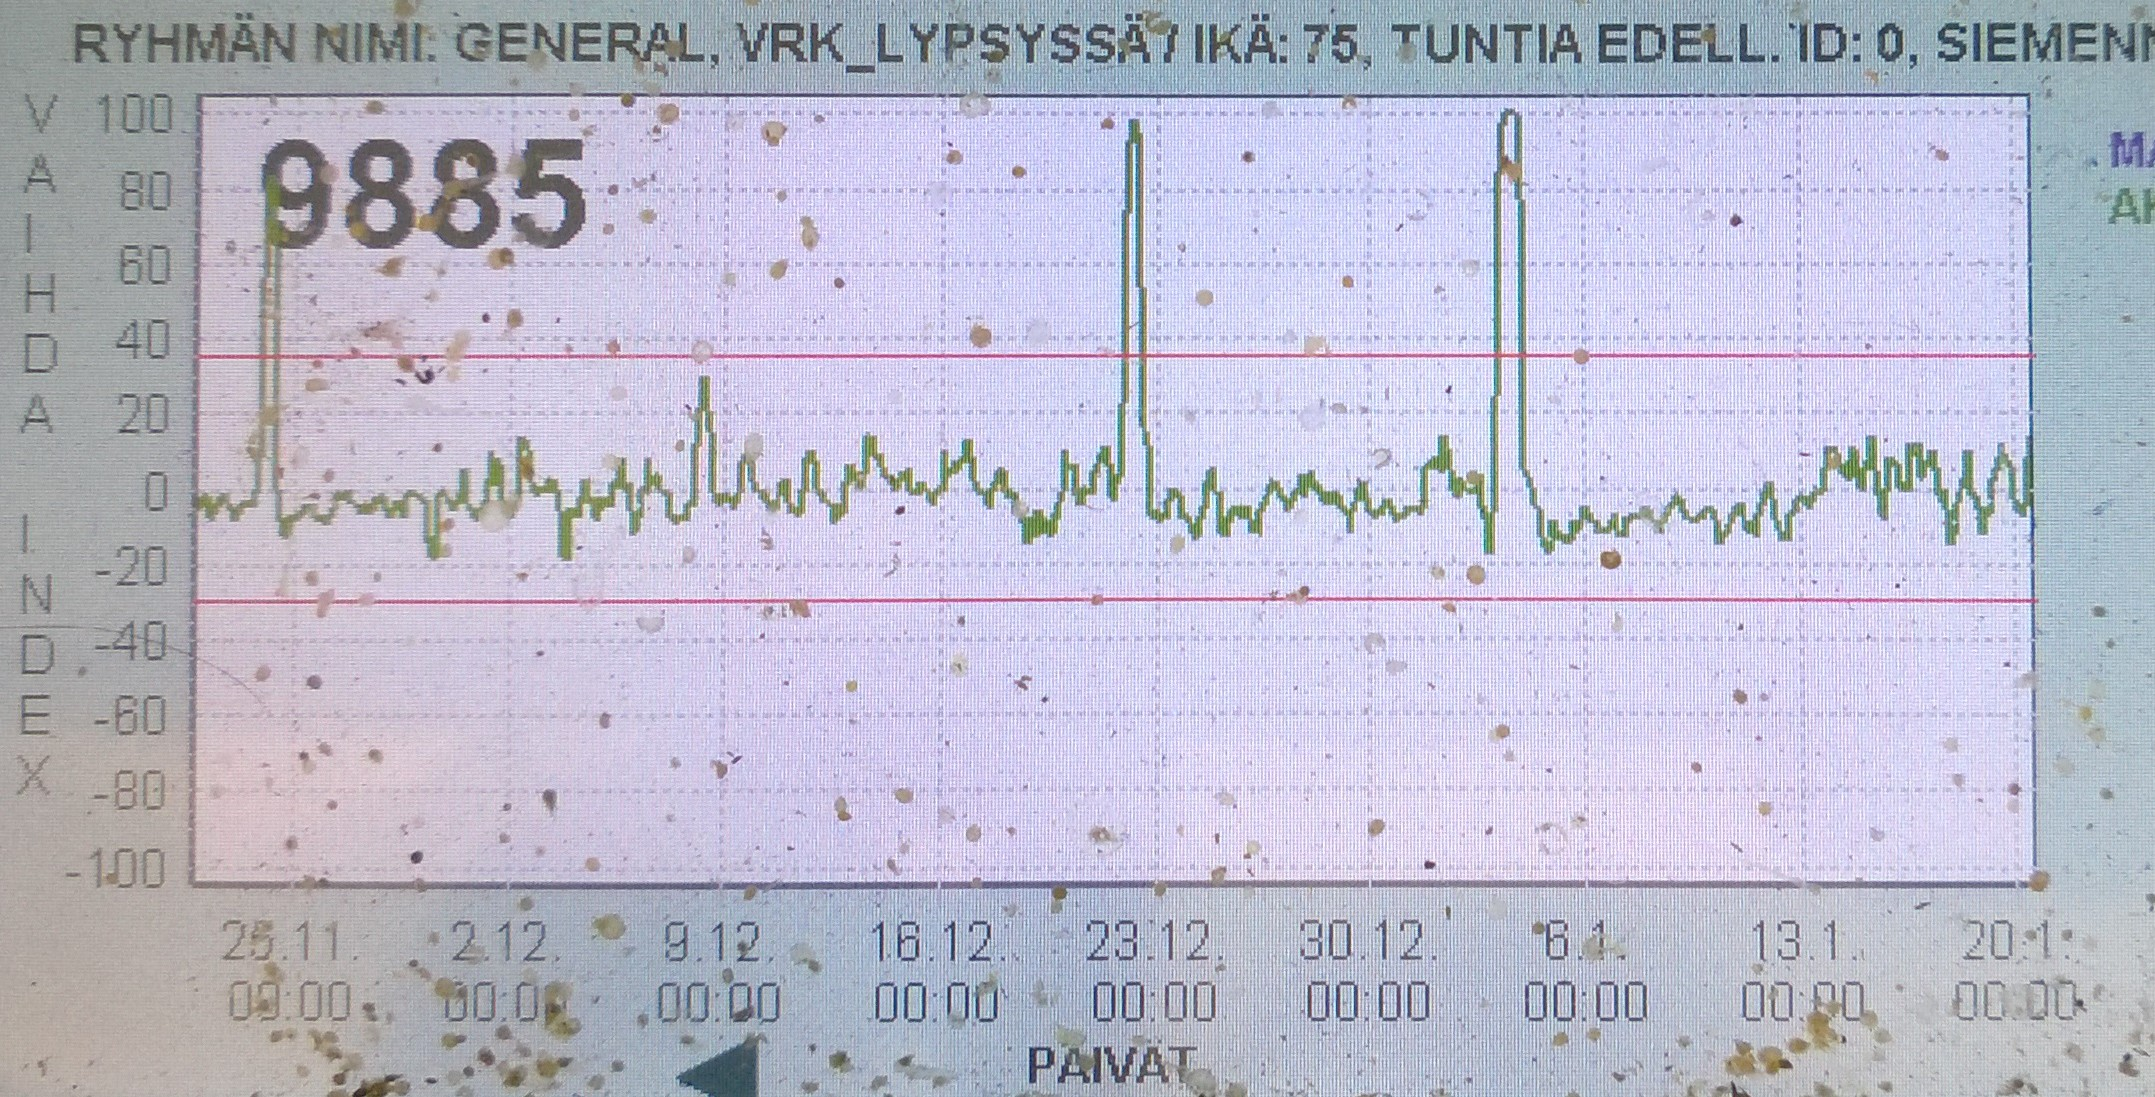
\includegraphics[width = 0.75\textwidth]{figures/heatime_kiima_9885}
\caption{The activity data of Heatime system of the cow 9885. The cow has had estruses approximately on October the 24\textsuperscript{th}, December the 22\textsuperscript{nd} and January the 4\textsuperscript{th}. Two latter estruses should be detectable in this study, hence they both are within our dat recording period. }
\label{heatime_kiima_9885}
\end{figure}

\begin{figure}[h]
\centering
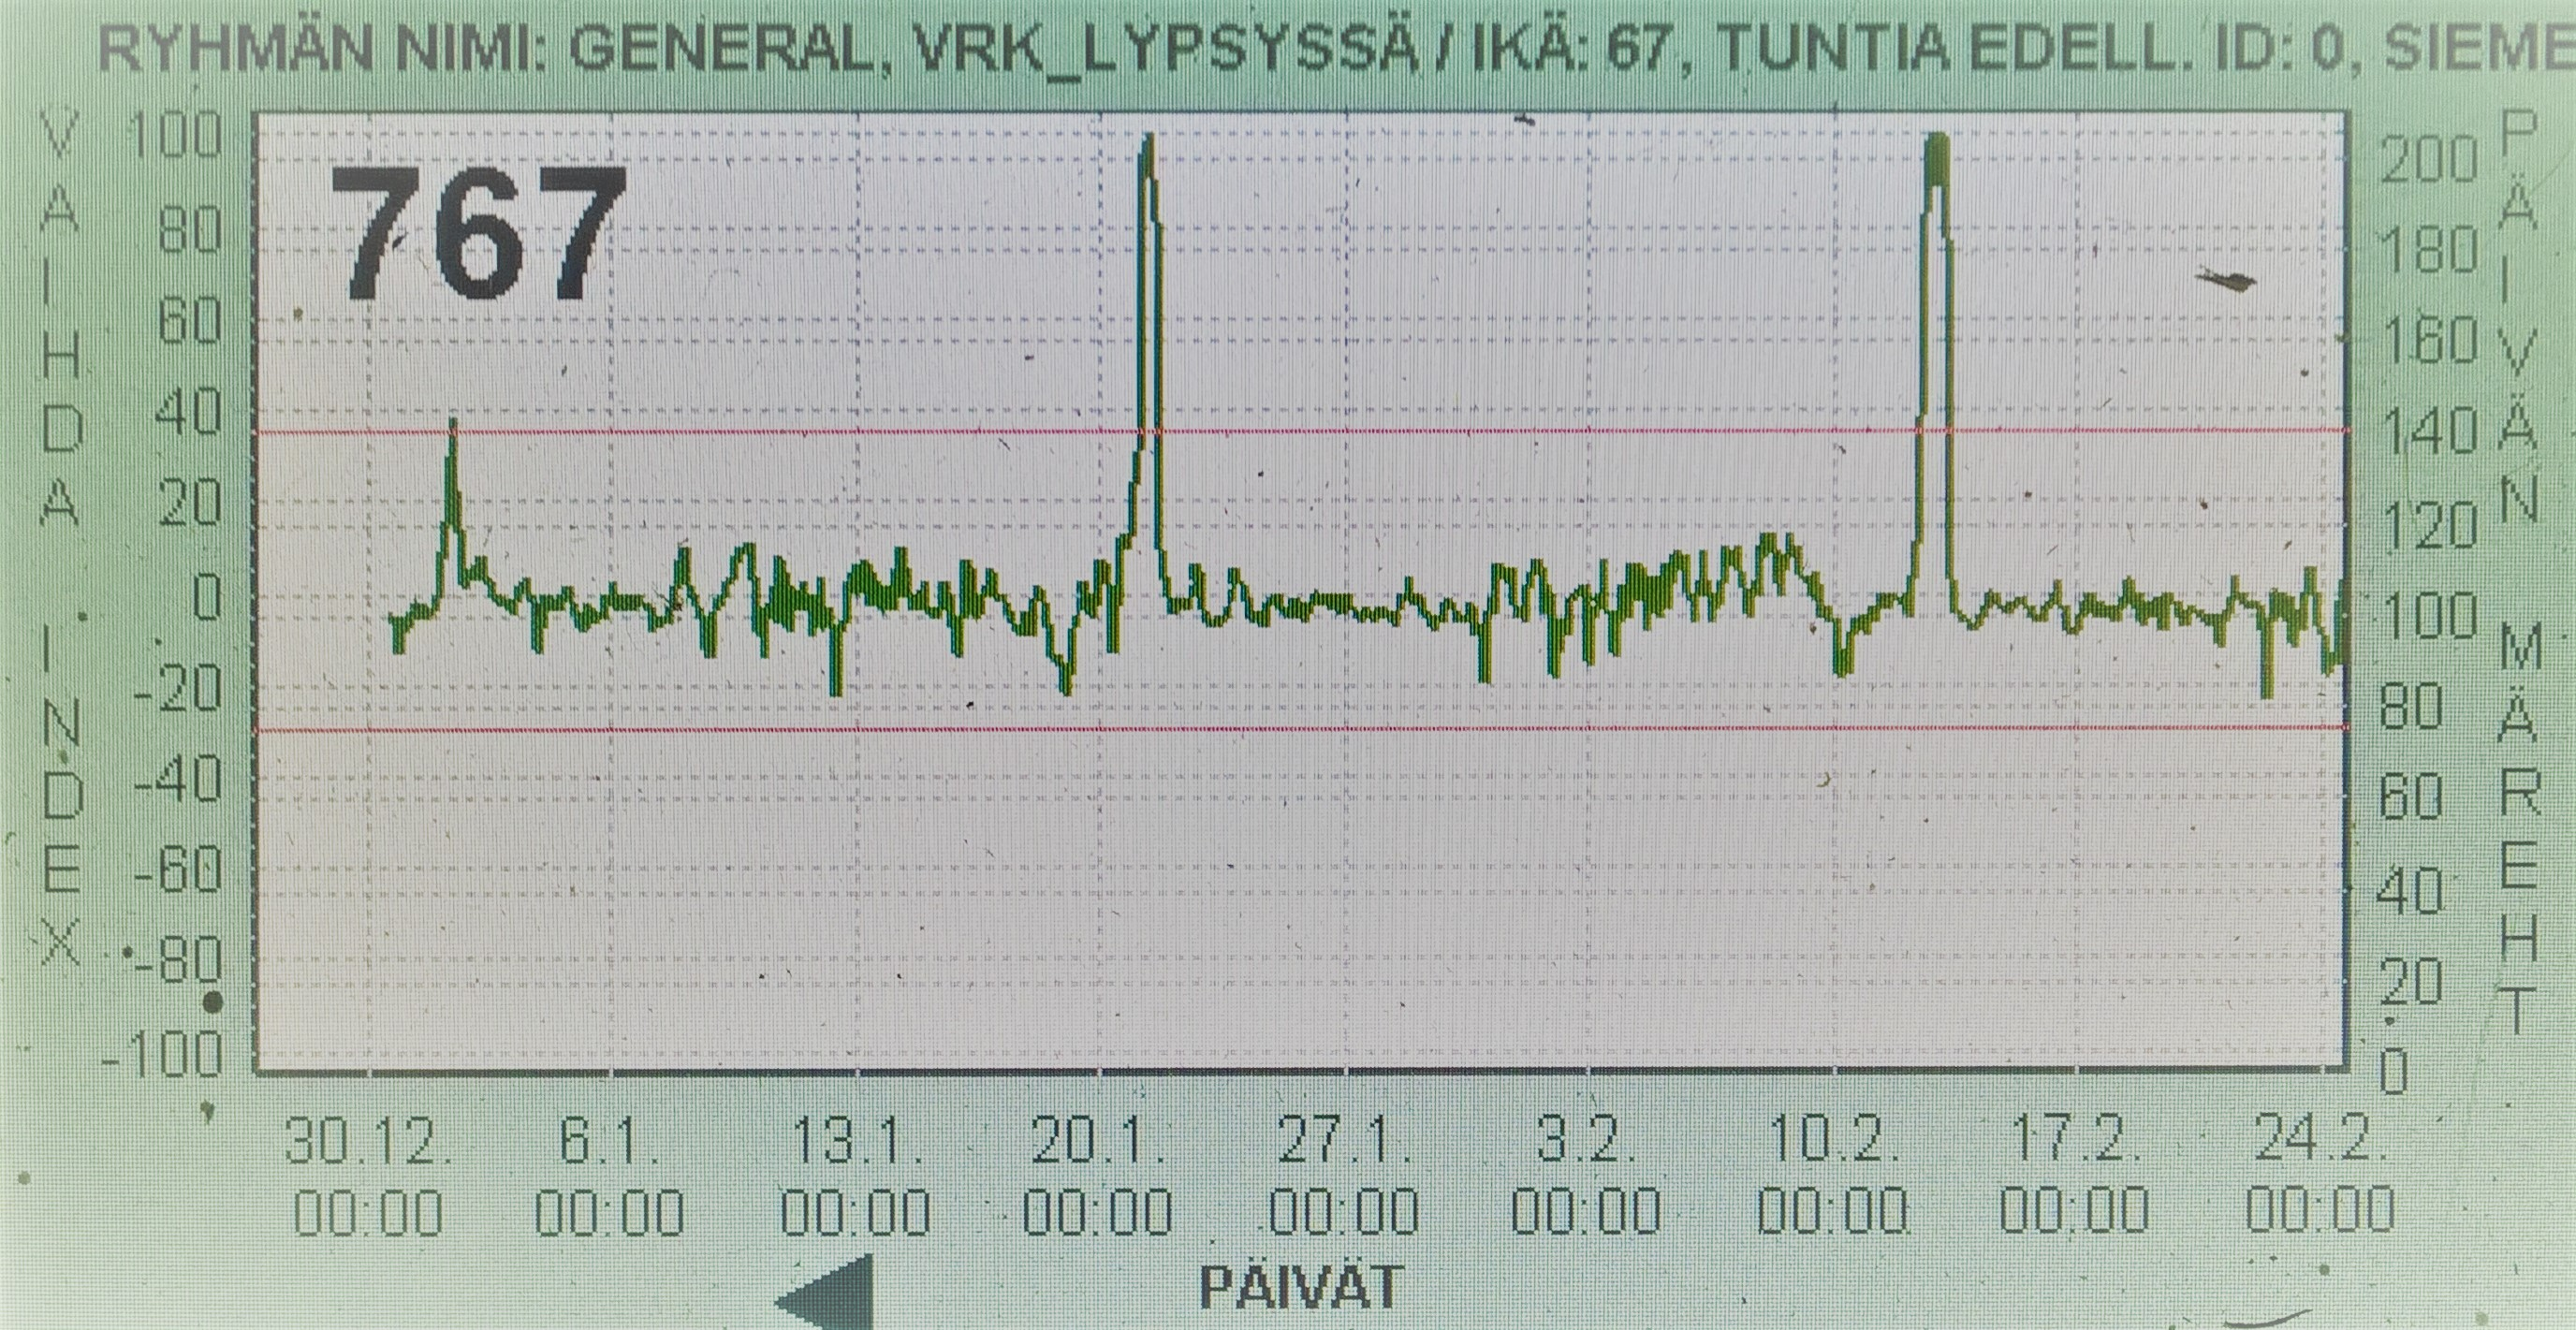
\includegraphics[width = 0.75\textwidth]{figures/heatime_kiima_767}
\caption{The activity data of Heatime system of the cow 767. The cow has had estruses approximately on January the 21\textsuperscript{st} and February the 13\textsuperscript{th}. The latter of the estruses should be detectable in this study, hence it is within our data recording period.}
\label{heatime_kiima_767_2}
\end{figure}

\begin{figure}[h]
\centering
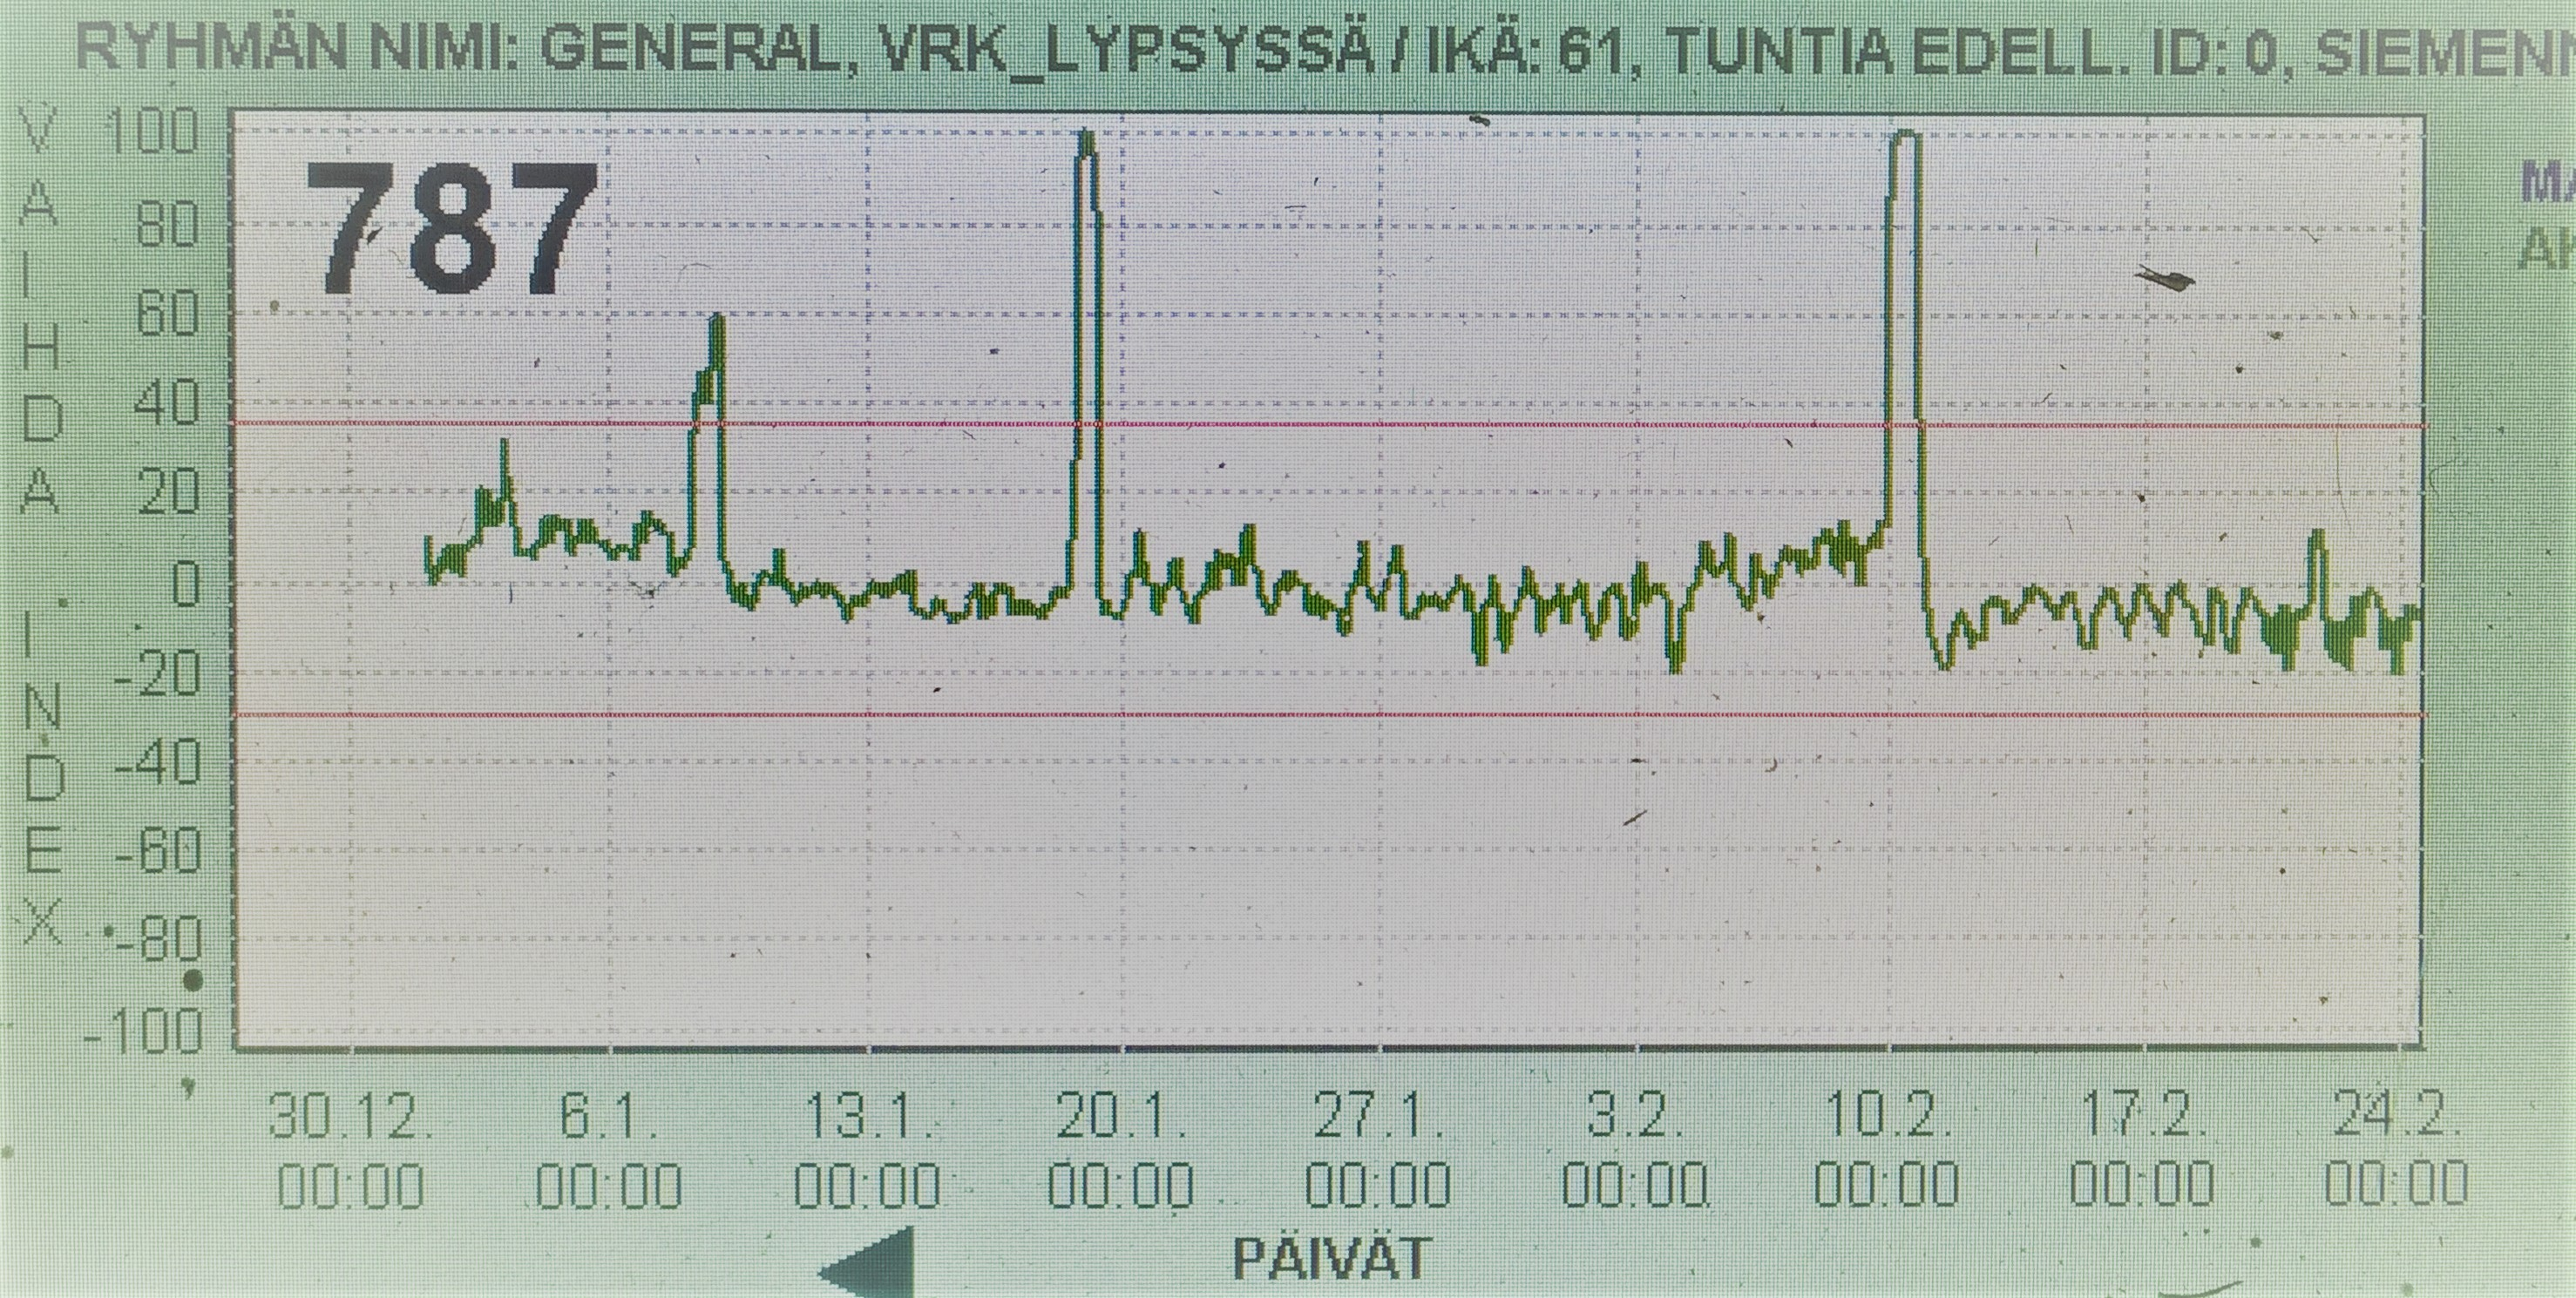
\includegraphics[width = 0.75\textwidth]{figures/heatime_kiima_787}
\caption{The activity data of Heatime system of the cow 787. The cow has had estruses approximately on January the 19\textsuperscript{th} and February the 10\textsuperscript{th}. The latter of the estruses should detectable in this study, hence it is within our data recording period.}
\label{heatime_kiima_787}
\end{figure}



\clearpage
\section{Raw Accelerometric Data}

\begin{figure}[h]
\centering
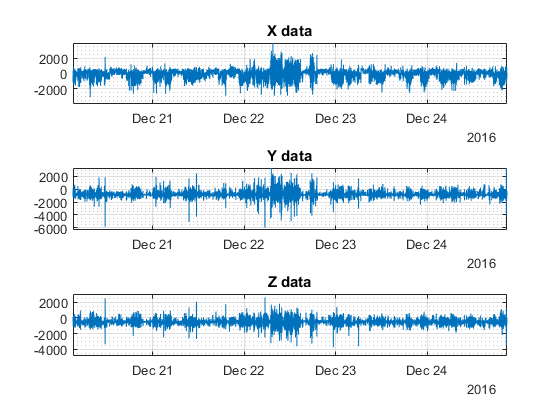
\includegraphics[width = 0.75\textwidth]{figures/kiimadata_9885_1.png}
\caption{The raw acceleration data of each axis of the cow 9885. The time frame is scaled around the first detectable estrus period. }
\label{kiimadata_9885_1}
\end{figure}

\begin{figure}[h]
\centering
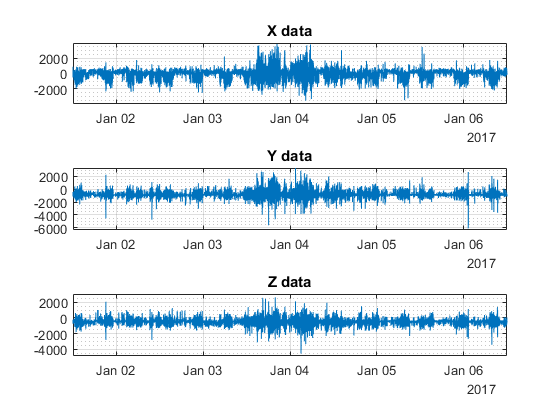
\includegraphics[width = 0.75\textwidth]{figures/kiimadata_9885_2.png}
\caption{The raw acceleration data of each axis of the cow 9885. The time frame is scaled around the second detectable estrus period. }
\label{kiimadata_9885_2}
\end{figure}

\clearpage
\section{Activity Monitoring Full Results}

\begin{figure}[h]
\centering
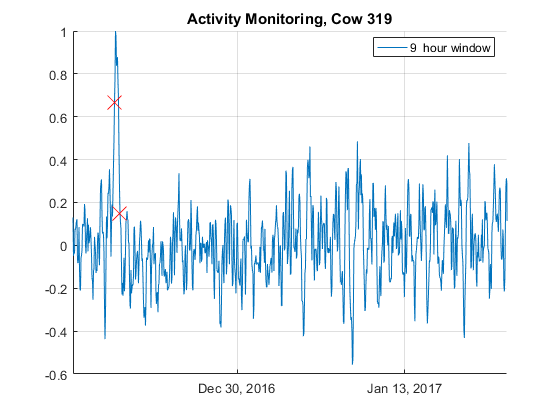
\includegraphics[width = 0.75 \textwidth]{figures/ActivityMonitoringCow319.png}
\caption{The plot of the results of the activity measurement algorithm of cow 319. A true positive estrus is detected and no false positive or false negative detection occurred. However, there is a lot of variation when not in estrus. Thus, the risk of false positive and false negative results is plausible.}
\label{ActivityMonitoringCow319}
\end{figure}

\begin{figure}[h]
\centering
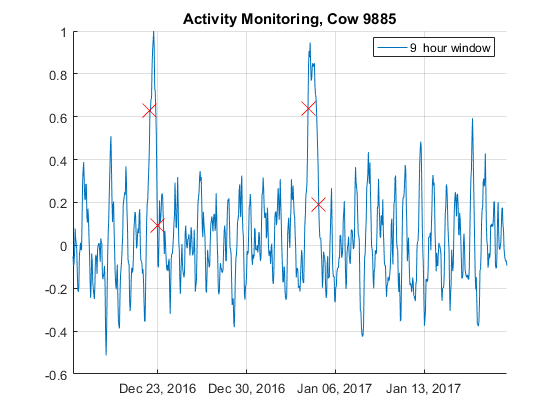
\includegraphics[width = 0.75 \textwidth]{figures/ActivityMonitoringCow9885.png}
\caption{The results of activity measurement of the cow 9885. Both of the estruses are detected. However, the difference between the estruses and the rest of the period is insignificant as it was with cow 319. Thus, the possibility of false positive and false negative results exists.}
\label{ActivityMonitoringCow9885}
\end{figure}

\begin{figure}[h]
\centering
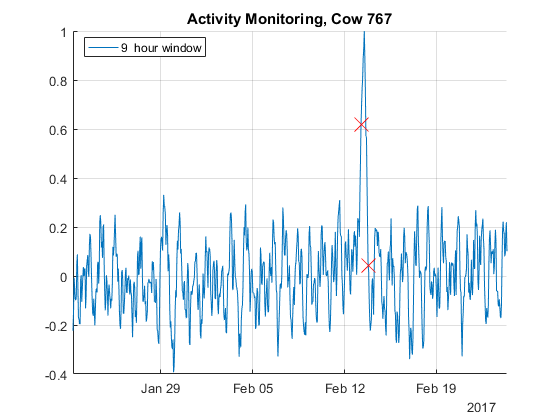
\includegraphics[width = 0.75 \textwidth]{figures/ActivityMonitoringCow767.png}
\caption{The plot of the activity measurement results of the cow 767. A true positive estrus is detected and no occurrence of false positives of false negatives. Additionally, the difference between proestrus and rest of the period is obvious. The risk of false positive or false negative results is minor. }
\label{ActivityMonitoringCow767}
\end{figure}

\begin{figure}[h]
\centering
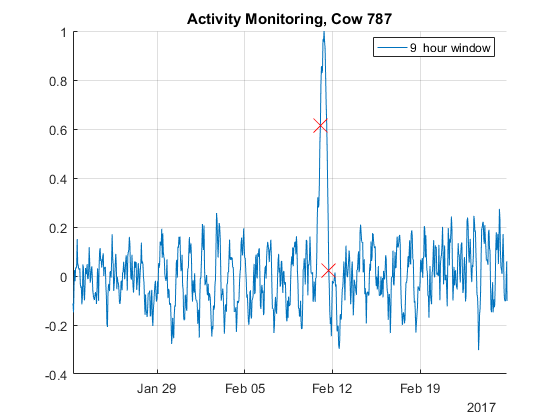
\includegraphics[width = 0.75 \textwidth]{figures/ActivityMonitoringCow787.png}
\caption{The results of activity measurement of the cow 787. The difference between the estrus and rest of the period is most distinct within this algorithm. Thus, the risk of false positive and false negative results is least significant.}
\label{ActivityMonitoringCow787}
\end{figure}

\begin{figure}[h]
\centering
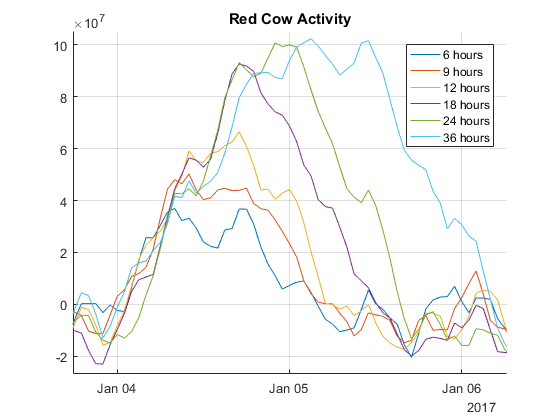
\includegraphics[width = 0.75\textwidth]{figures/redcowactivity2.png}
\caption{The activity plots of the second proestrus of the cow 9885. The figure illustrates the affect of varying the size of the integration window. Wider window increases the amplitude of the estrus and eases the detectability. However, simultaneously it delays the moment of detection. }
\label{integrationwindows}
\end{figure}

\clearpage
\section{Variance Detection Full Results}

\begin{figure}[h]
\centering
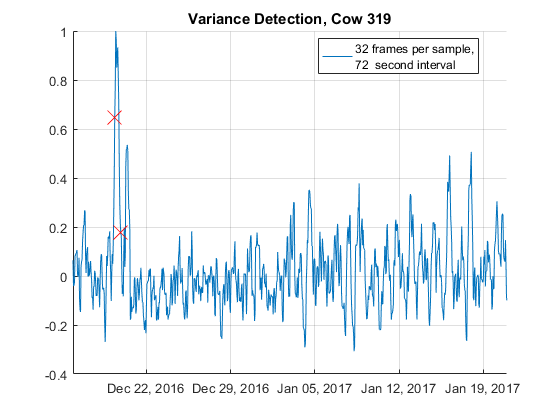
\includegraphics[width = 0.75 \textwidth]{figures/VarianceDetectionCow319.png}
\caption{The results of the variance detection algorithm of the cow 319. The estrus on December the 20\textsuperscript{th} is barely detectable. Additionally, algorithm yielded several false positive estruses. Furthermore, the amplitude of the false positives exceeds the true positive.}
\label{VarianceDetectionCow319}
\end{figure}

\begin{figure}[h]
\centering
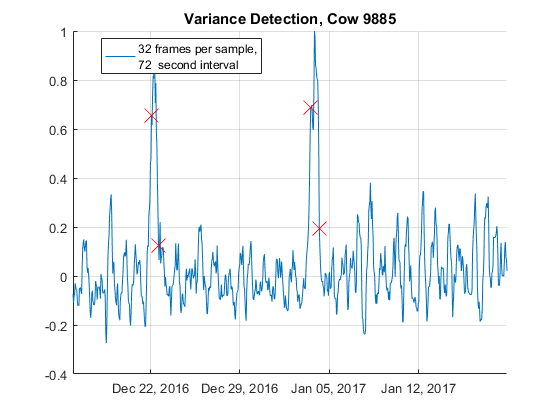
\includegraphics[width = 0.75 \textwidth]{figures/VarianceDetectionCow9885.png}
\caption{The results of variance detection algorithm of the cow 9885. The true positive estrus is detected on December the 22\textsuperscript{st}. Furthermore, the amplitude difference between the detected estrus and other period is significant. However, the algorithm yield a false negative on January the 4\textsuperscript{th}.}
\label{VarianceDetectionCow9885}
\end{figure}

\begin{figure}[h]
\centering
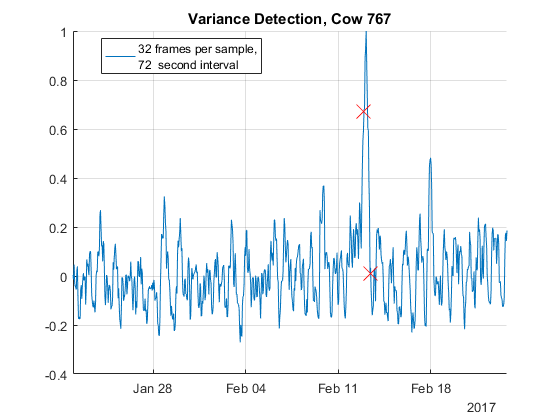
\includegraphics[width = 0.75 \textwidth]{figures/VarianceDetectionCow767.png}
\caption{The variance detection results of the cow 767. There are multiple false positive detections in the data period. In general, there is no obvious difference between the estrus and non-estrus periods. Nevertheless, a true positive estrus is detected on February the 13\textsuperscript{th}.}
\label{VarianceDetectionCow767}
\end{figure}

\begin{figure}[h]
\centering
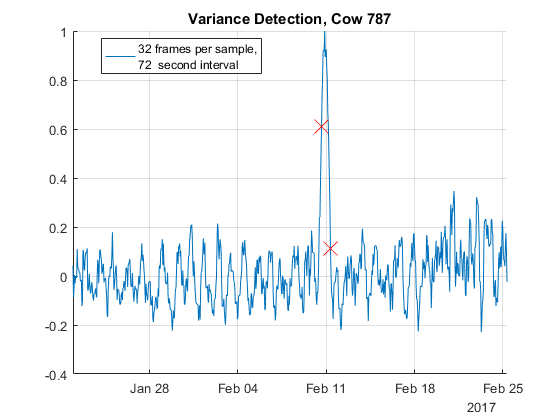
\includegraphics[width = 0.75 \textwidth]{figures/VarianceDetectionCow787.png}
\caption{The results of variance detection algorithm of the cow 787. The true positive estrus is detected on February the 10\textsuperscript{th}. However, a false positive detection occurred on February the 21\textsuperscript{st}. Otherwise, the amplitude  difference between estrus and non-estrus periods is obvious.}
\label{VarianceDetectionCow787}
\end{figure}

\begin{figure}[h]
\centering
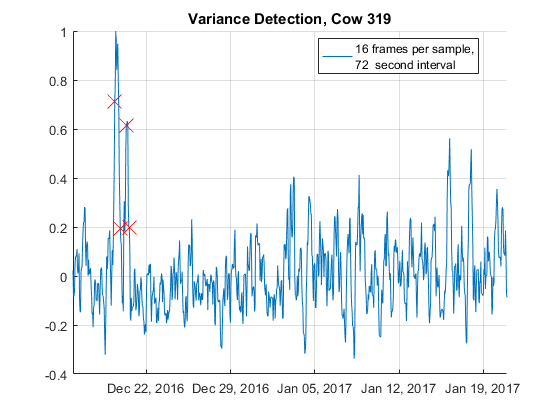
\includegraphics[width = 0.75 \textwidth]{figures/VarianceDetectionCow319_16frames72seconds.png}
\caption{Reducing the sample size to 16 frames per sample and keeping the sampling interval in 72 seconds yields false positive results with the cow 319}
\label{}
\end{figure}

\begin{figure}[h]
\centering
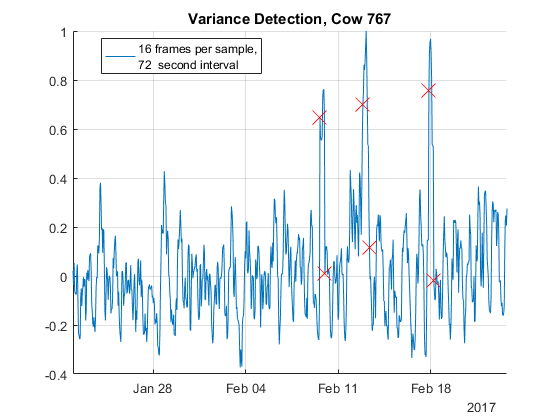
\includegraphics[width = 0.75 \textwidth]{figures/VarianceDetectionCow767_16frames72seconds.png}
\caption{Reducing the sample size to 16 frames per sample and keeping the sampling interval in 72 seconds yields false positive results with the cow 767}
\label{}
\end{figure}

%------------%

\begin{figure}[h]
\centering
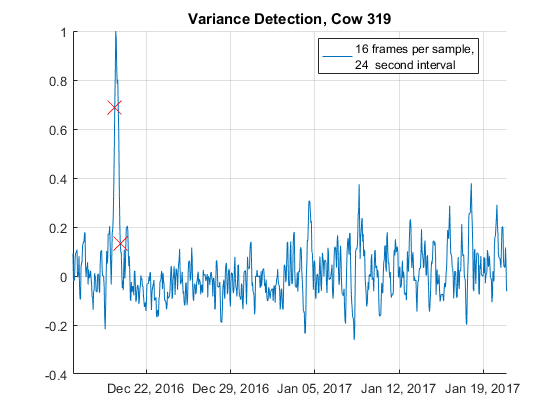
\includegraphics[width = 0.75 \textwidth]{figures/VarianceDetectionCow319_16frames24seconds.png}
\caption{Reducing the sample size to 16 frames and increasing the sampling interval to 24 seconds improves the performance of the variance detection algorithm. Consequently, no false positive results occurs.}
\label{}
\end{figure}

\begin{figure}[h]
\centering
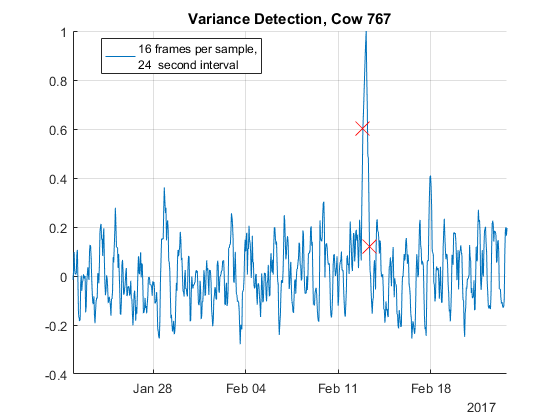
\includegraphics[width = 0.75 \textwidth]{figures/VarianceDetectionCow767_16frames24seconds.png}
\caption{Reducing the sample size to 16 frames and increasing the sampling interval to 24 seconds improves the performance of the variance detection algorithm. Consequently, no false positive results occurs.}
\label{}
\end{figure}


Varying the sampling interval affect the results:


\begin{figure}[h]
\centering
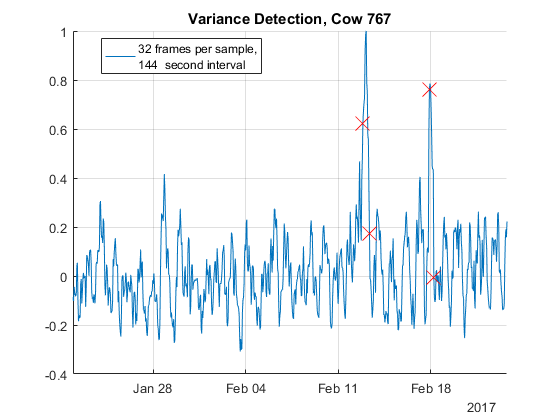
\includegraphics[width = 0.75 \textwidth]{figures/VarianceDetectionCow767_32frames144seconds.png}
\caption{More seldom sampling yield false positive results as seen in this picture.}
\label{}
\end{figure}


\begin{figure}[h]
\centering
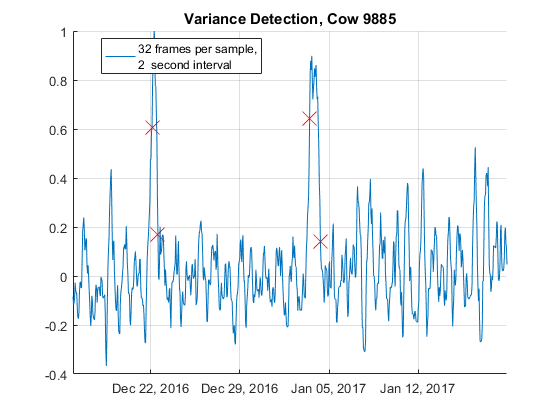
\includegraphics[width = 0.75 \textwidth]{figures/VarianceDetectionCow9885_32frames2seconds.png}
\caption{Decreasing the sampling interval does not directly improve the results as it is with the cow 9885. This sampling frequency corresponds approximately continuous sampling. Nevertheless, the results are worse than formerly.}
\label{}
\end{figure}



\begin{figure}[h]
\centering
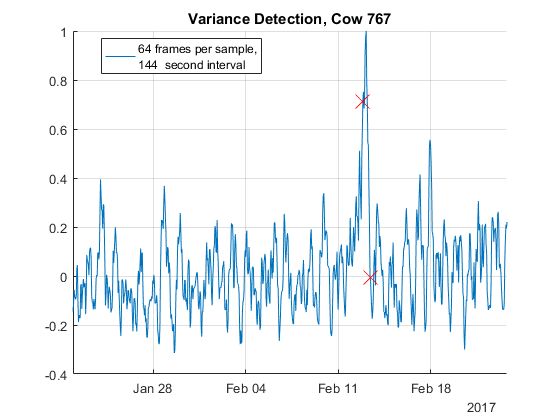
\includegraphics[width = 0.75 \textwidth]{figures/VarianceDetectionCow767_64frames144seconds.png}
\caption{}
\label{}
\end{figure}

\begin{figure}[htb]
\centering
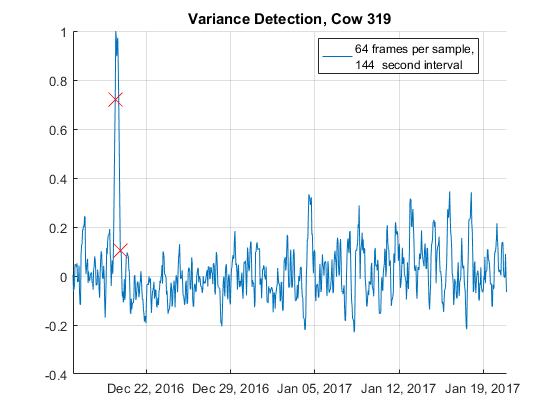
\includegraphics[width = 0.75 \textwidth]{figures/VarianceDetectionCow319_64frames144seconds.png}
\caption{}
\label{}
\end{figure}

\begin{figure}[h]
\centering
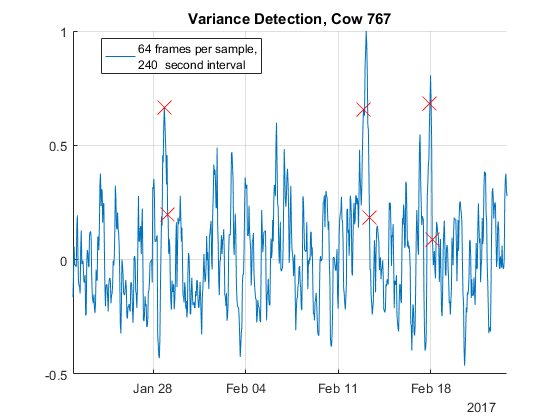
\includegraphics[width = 0.75 \textwidth]{figures/VarianceDetectionCow767_64frames240seconds.png}
\caption{}
\label{}
\end{figure}


\clearpage
\section{Inactivity Detection Full Results}


\begin{figure}[h]
\centering
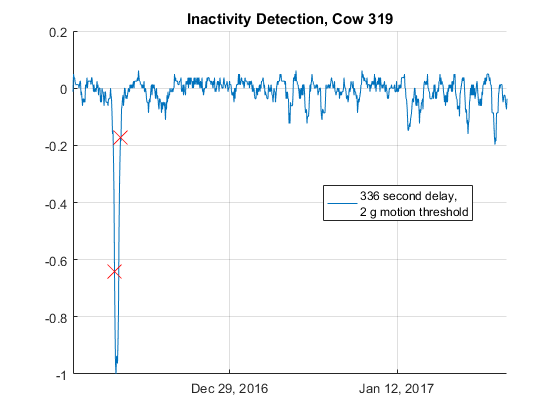
\includegraphics[width = 0.75 \textwidth]{figures/InactivityDetectionCow319.png}
\caption{The results of the inactivity detection algorithm of the cow 319. The parameters are 336 second delay and \SI{2}{\gram} motion threshold. A true positive estrus is detected on December the 20\textsuperscript{th}. The amplitude of proestrus and non-estrus is significant. }
\label{InactivityDetectionCow319}
\end{figure}


\begin{figure}[h]
\centering
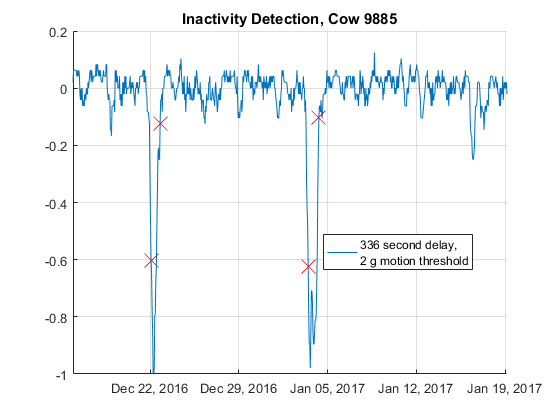
\includegraphics[width = 0.75 \textwidth]{figures/InactivityDetectionCow9885.png}
\caption{The results of inactivity detection algorithm of the cow 9885. The parameters are 336 second delay and \SI{2}{\gram} motion threshold. Both of the estruses are detected as true positive on December the 22\textsuperscript{nd} and January the 4\textsuperscript{th}. No false positive or false negative detection occurred. The amplitude difference between proestrus and non-estrus is obvious.}
\label{InactivityDetectionCow9885}
\end{figure}


\begin{figure}[h]
\centering
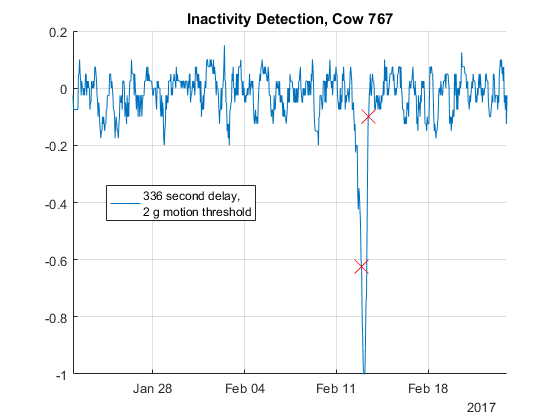
\includegraphics[width = 0.75 \textwidth]{figures/InactivityDetectionCow767.png}
\caption{The results of the inactivity detection algorithm of the cow 767. The parameters are 336 second delay and \SI{2}{\gram} motion threshold. A true positive estrus is detected on February the 13\textsuperscript{th}. Additionally, the amplitude of the proestrus differs from none-estrus significantly.}
\label{InactivityDetectionCow767}
\end{figure}

\begin{figure}[h]
\centering
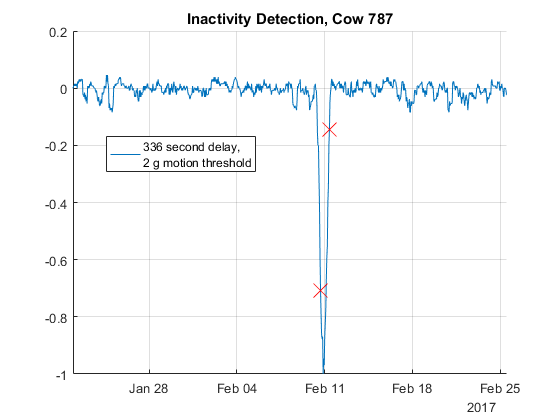
\includegraphics[width = 0.75 \textwidth]{figures/InactivityDetectionCow787.png}
\caption{The results of inactivity detection algorithm of the cow 787. The parameters are 336 second delay and \SI{2}{\gram} motion threshold. A ture positive estrus is detected on February the 11\textsuperscript{th} and no false positives of false negatives occurred. Furthermore, the difference between estrus and other periods is most significant.}
\label{InactivityDetectionCow787}
\end{figure}



\begin{figure}[h]
\centering
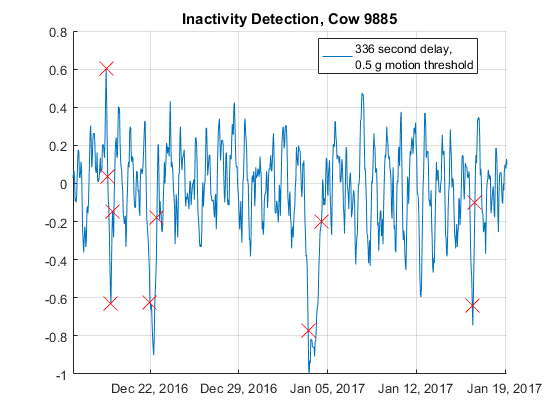
\includegraphics[width = 0.75 \textwidth]{figures/InactivityDetectionCow9885_336period05threshold.png}
\caption{}
\label{}
\end{figure}

\begin{figure}[h]
\centering
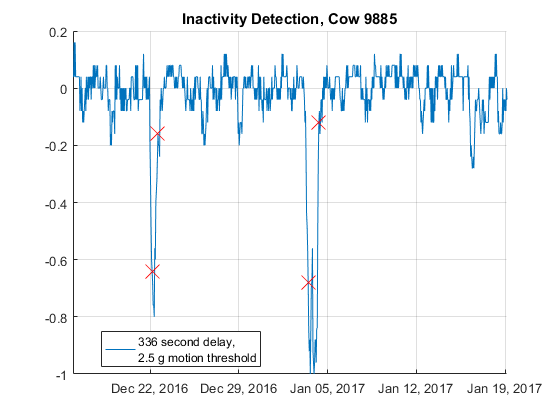
\includegraphics[width = 0.75 \textwidth]{figures/InactivityDetectionCow9885_336period2_5threshold.png}
\caption{}
\label{}
\end{figure}

\begin{figure}[h]
\centering
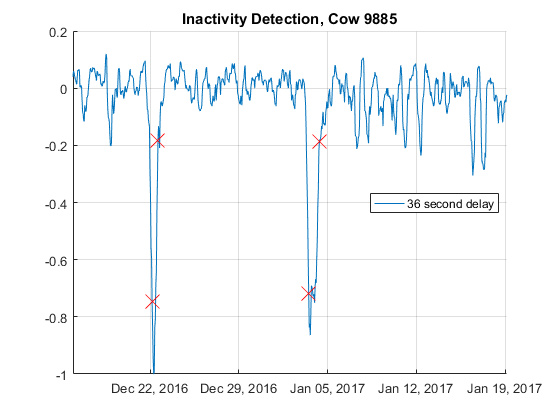
\includegraphics[width = 0.75 \textwidth]{figures/InactivityDetectionCow9885_36period.png}
\caption{}
\label{}
\end{figure}

\begin{figure}[h]
\centering
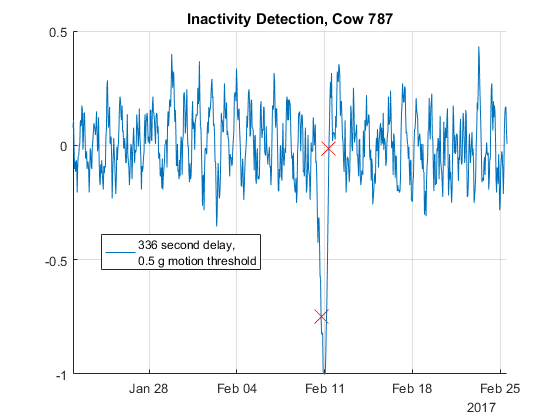
\includegraphics[width = 0.75 \textwidth]{figures/InactivityDetectionCow787_336period05threshold.png}
\caption{}
\label{}
\end{figure}

\begin{figure}[h]
\centering
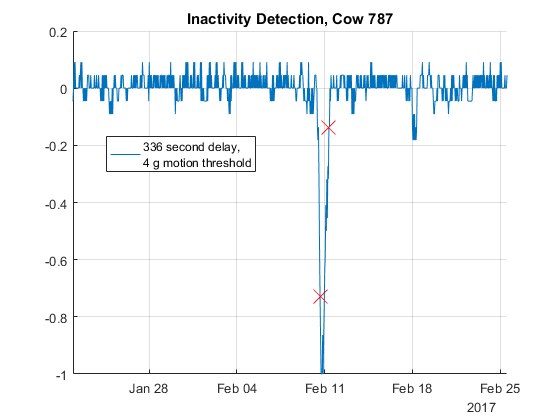
\includegraphics[width = 0.75 \textwidth]{figures/InactivityDetectionCow787_336period4threshold.png}
\caption{}
\label{}
\end{figure}

\begin{figure}[h]
\centering
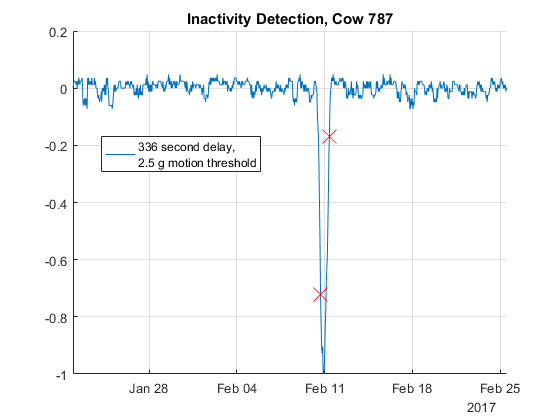
\includegraphics[width = 0.75 \textwidth]{figures/InactivityDetectionCow787_336period2_5threshold.png}
\caption{}
\label{}
\end{figure}

\begin{figure}[h]
\centering
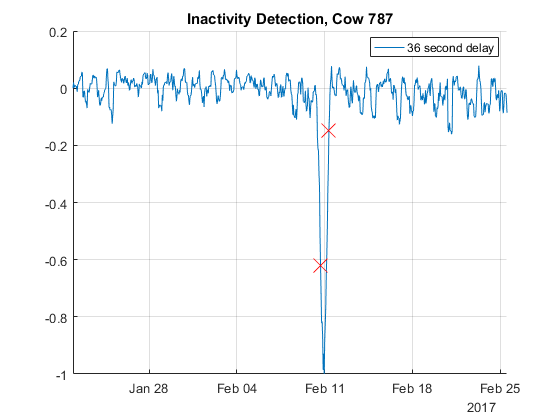
\includegraphics[width = 0.75 \textwidth]{figures/InactivityDetectionCow787_36period.png}
\caption{}
\label{}
\end{figure}

\begin{figure}[h]
\centering
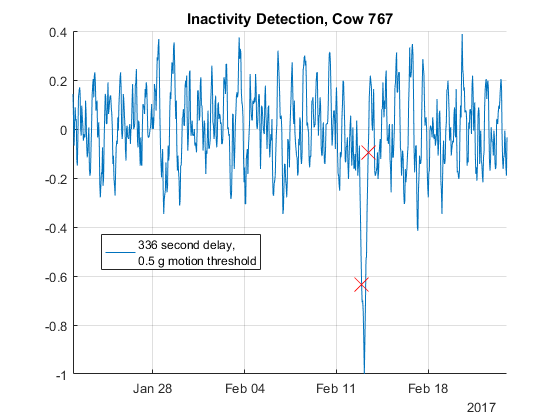
\includegraphics[width = 0.75 \textwidth]{figures/InactivityDetectionCow767_336period05threshold.png}
\caption{}
\label{}
\end{figure}

\begin{figure}[h]
\centering
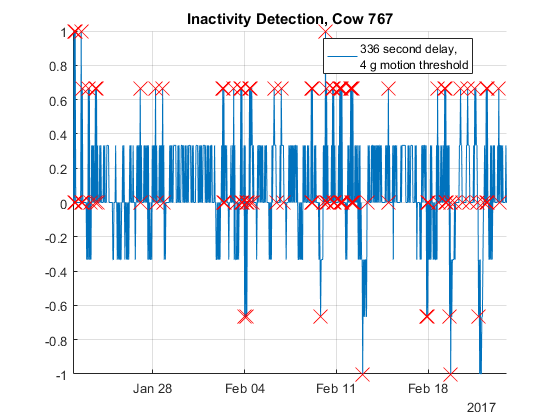
\includegraphics[width = 0.75 \textwidth]{figures/InactivityDetectionCow767_336period4threshold.png}
\caption{}
\label{}
\end{figure}


\begin{figure}[h]
\centering
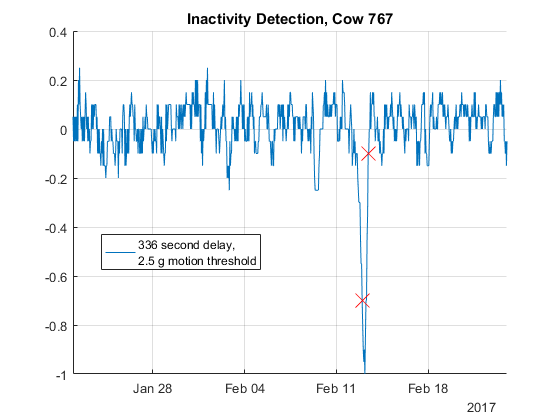
\includegraphics[width = 0.75 \textwidth]{figures/InactivityDetectionCow767_336period2_5threshold.png}
\caption{}
\label{}
\end{figure}

\begin{figure}[h]
\centering
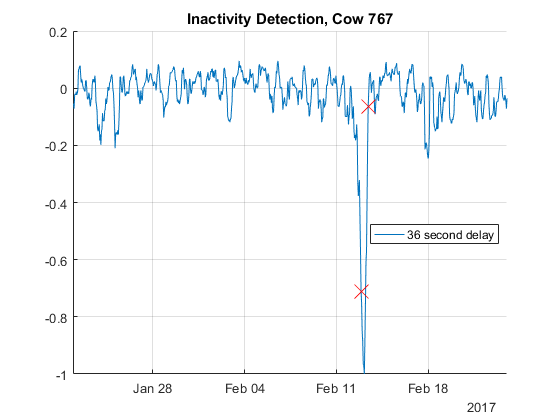
\includegraphics[width = 0.75 \textwidth]{figures/InactivityDetectionCow767_36period.png}
\caption{}
\label{}
\end{figure}

\begin{figure}[h]
\centering
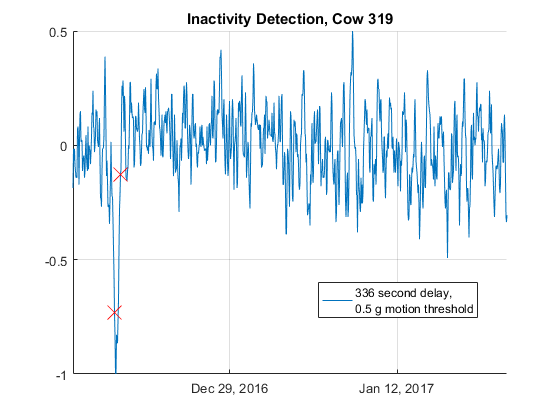
\includegraphics[width = 0.75 \textwidth]{figures/InactivityDetectionCow319_336period05threshold.png}
\caption{}
\label{}
\end{figure}

\begin{figure}[h]
\centering
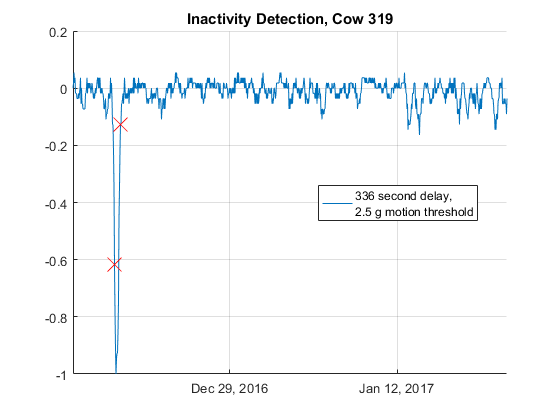
\includegraphics[width = 0.75 \textwidth]{figures/InactivityDetectionCow319_336period2_5threshold.png}
\caption{}
\label{}
\end{figure}

\begin{figure}[h]
\centering
\includegraphics[width = 0.75 \textwidth]{figures/InactivityDetectionCow319_36period.png}
\caption{}
\label{}
\end{figure}




%
%\section{Esimerkki liitteestä\label{LiiteA}}
%
%Liitteet eivät ole opinnäytteen kannalta välttämättömiä ja 
%opinnäytteen tekijän on 
%kirjoittamaan ryhtyessään hyvä ajatella pärjäävänsä ilman liitteitä.
%Kokemattomat kirjoittajat, jotka ovat huolissaan
%tekstiosan pituudesta, paisuttavat turhan 
%helposti liitteitä pitääkseen tekstiosan pituuden annetuissa rajoissa.
%Tällä tavalla ei synny hyvää opinnäytettä.   
%
%Liite on itsenäinen kokonaisuus, vaikka se täydentääkin tekstiosaa.
%Liite ei siten ole pelkkä listaus, kuva tai taulukko, vaan 
%liitteessä selitetään aina sisällön laatu ja tarkoitus. 
%
%Liitteeseen voi laittaa esimerkiksi listauksia. Alla on 
%listausesimerkki tämän liitteen luomisesta. 
%
%%% Verbatim-ympäristö ei muotoile tai tavuta tekstiä. Fontti on monospace.
%%% Verbatim-ympäristön sisällä annettuja komentoja ei LaTeX käsittele. 
%%% Vasta \end{verbatim}-komennon jälkeen jatketaan käsittelyä.
%\begin{verbatim}
%	\clearpage
%	\appendix
%	\addcontentsline{toc}{section}{Liite A}
%	\section*{Liite A}
%	...
%	\thispagestyle{empty}
%	...
%	tekstiä
%	...
%	\clearpage
%\end{verbatim}
%
%Kaavojen numerointi muodostaa liitteissä oman kokonaisuutensa:
%\begin{eqnarray}
%d \wedge A  &=& F, \label{liitekaava1}\\
%d \wedge F  &=& 0. \label{liitekaava2}
%\end{eqnarray}
%
%
%\clearpage
%\section{Toinen esimerkki liitteestä\label{LiiteB}}
%
%%% Liitteiden kaavat, taulukot ja kuvat numeroidaan omana kokonaisuutenaan
%
%Liitteissä voi myös olla kuvia, jotka
%eivät sovi leipätekstin joukkoon:
%%% Ympäristön figure parametrit htb pakottavat
%%% kuvan tähän, eikä LaTeX yritä siirrellä niitä
%%% hyväksi katsomaansa paikkaan. 
%%% Ympäristöä center voi käyttää \centering-
%%% komennon sijaan
%%%
%\begin{figure}[htb]
%\begin{center}
%\includegraphics[height=8cm]{kuva2}
%\end{center}
%\caption{Kuvateksti, jossa on liitteen numerointi}
%\label{liitekuva}
%\end{figure}
%%%
%Liitteiden taulukoiden numerointi on kuvien ja kaavojen kaltainen:
%\begin{table}[htb]
%\caption{Taulukon kuvateksti.}
%\label{liitetaulukko}
%\begin{center}
%\fbox{
%\begin{tabular}{lp{0.5\linewidth}}
%9.00--9.55  & Käytettävyystestauksen tiedotustilaisuus (osanottajat
%ovat saaneet sähköpostitse valmistautumistehtävät, joten tiedotustilaisuus
%voidaan pitää lyhyenä).\\
%9.55--10.00 & Testausalueelle siirtyminen
%\end{tabular}}
%\end{center}
%\end{table}
%Kaavojen numerointi muodostaa liitteissä oman kokonaisuutensa:
%\begin{eqnarray}
%T_{ik} &=& -p g_{ik} + w u_i u_k + \tau_{ik},  \label{liitekaava3} \\
%n_i    &=& n u_i + v_i.                      \label{liitekaava4}
%\end{eqnarray}


\end{document}
